\documentclass[10pt]{beamer}
\usetheme{Madrid}
\usepackage[utf8]{inputenc}
\usepackage[french]{babel}
\usepackage[T1]{fontenc}
\usepackage{amsmath}
\usepackage{amsfonts}
\usepackage{amssymb}
\usepackage{graphicx}
\usepackage{relsize}
\usepackage{subcaption}
\usepackage{amsmath}
\usepackage{listings}
\usepackage{xcolor}
\usepackage{multicol}

\author{TRAN-THUONG Tien-Thinh}
\date{2021-2022}
% \title{Reconnaissance vocale lors d’appel d’urgence grâce à un réseau de neurones}
\title{Présentation}
\graphicspath{{Affiche/0-ReconnaissanceVocale/}{Affiche/1-Introduction/}{Affiche/2-Activation-Gradient/}{Affiche/4-XOR/}{Affiche/5-MNIST/}{Affiche/6-Mot/}{Affiche/7-Vocal/}}
\lstset{inputpath={Affiche/99-Code/}}
\newcommand{\norme}[1]{\| #1 \|}

\definecolor{codegreen}{rgb}{0,0.6,0}
\definecolor{codegray}{rgb}{0.5,0.5,0.5}
\definecolor{codepurple}{rgb}{0.58,0,0.82}
\definecolor{backcolour}{rgb}{0.95,0.95,0.92}
\lstdefinestyle{mystyle}{
    backgroundcolor=\color{backcolour},   
    commentstyle=\color{codegreen},
    keywordstyle=\color{magenta},
    numberstyle=\tiny\color{codegray},
    stringstyle=\color{codepurple},
    basicstyle=\ttfamily\footnotesize,
    breakatwhitespace=false,         
    breaklines=true,                 
    captionpos=b,                    
    keepspaces=true,                 
    numbers=left,                    
    numbersep=5pt,                  
    showspaces=false,                
    showstringspaces=false,
    showtabs=false,                  
    tabsize=2
}
\lstset{style=mystyle}

\begin{document}

\begin{frame}
\titlepage
\end{frame}

\begin{frame}{Problématique}
\begin{alert}{D'après le ministère de la Santé : }
Il y a eu plus de \textbf{31 millions} d'appels d'urgence en 2018. Seuls \textbf{69\%} des appels étaient décrochés dans la minute.
\end{alert}
\begin{block}{Objectif}
Utiliser la reconnaissance vocale par réseau de neurones pour aider à classifier rapidement l'objet d'un appel.
\end{block}
\end{frame}


\begin{frame}{La reconnaissance automatique de la parole}
\begin{itemize}
	\item[1] Le traitement acoustique 
	\item[2] L'apprentissage automatique
	\item[3] Le décodage
\end{itemize}
\begin{figure}
	\begin{subfigure}[]{0.3\textwidth}
		\centering
		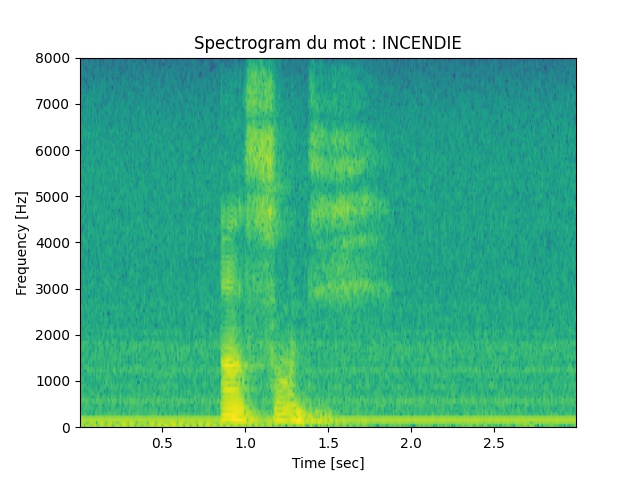
\includegraphics[height=50px]{1-Incendie-3.jpg}
  		\caption{Spectrogramme}
	\end{subfigure}
	\begin{subfigure}[]{0.3\textwidth}
		\centering
		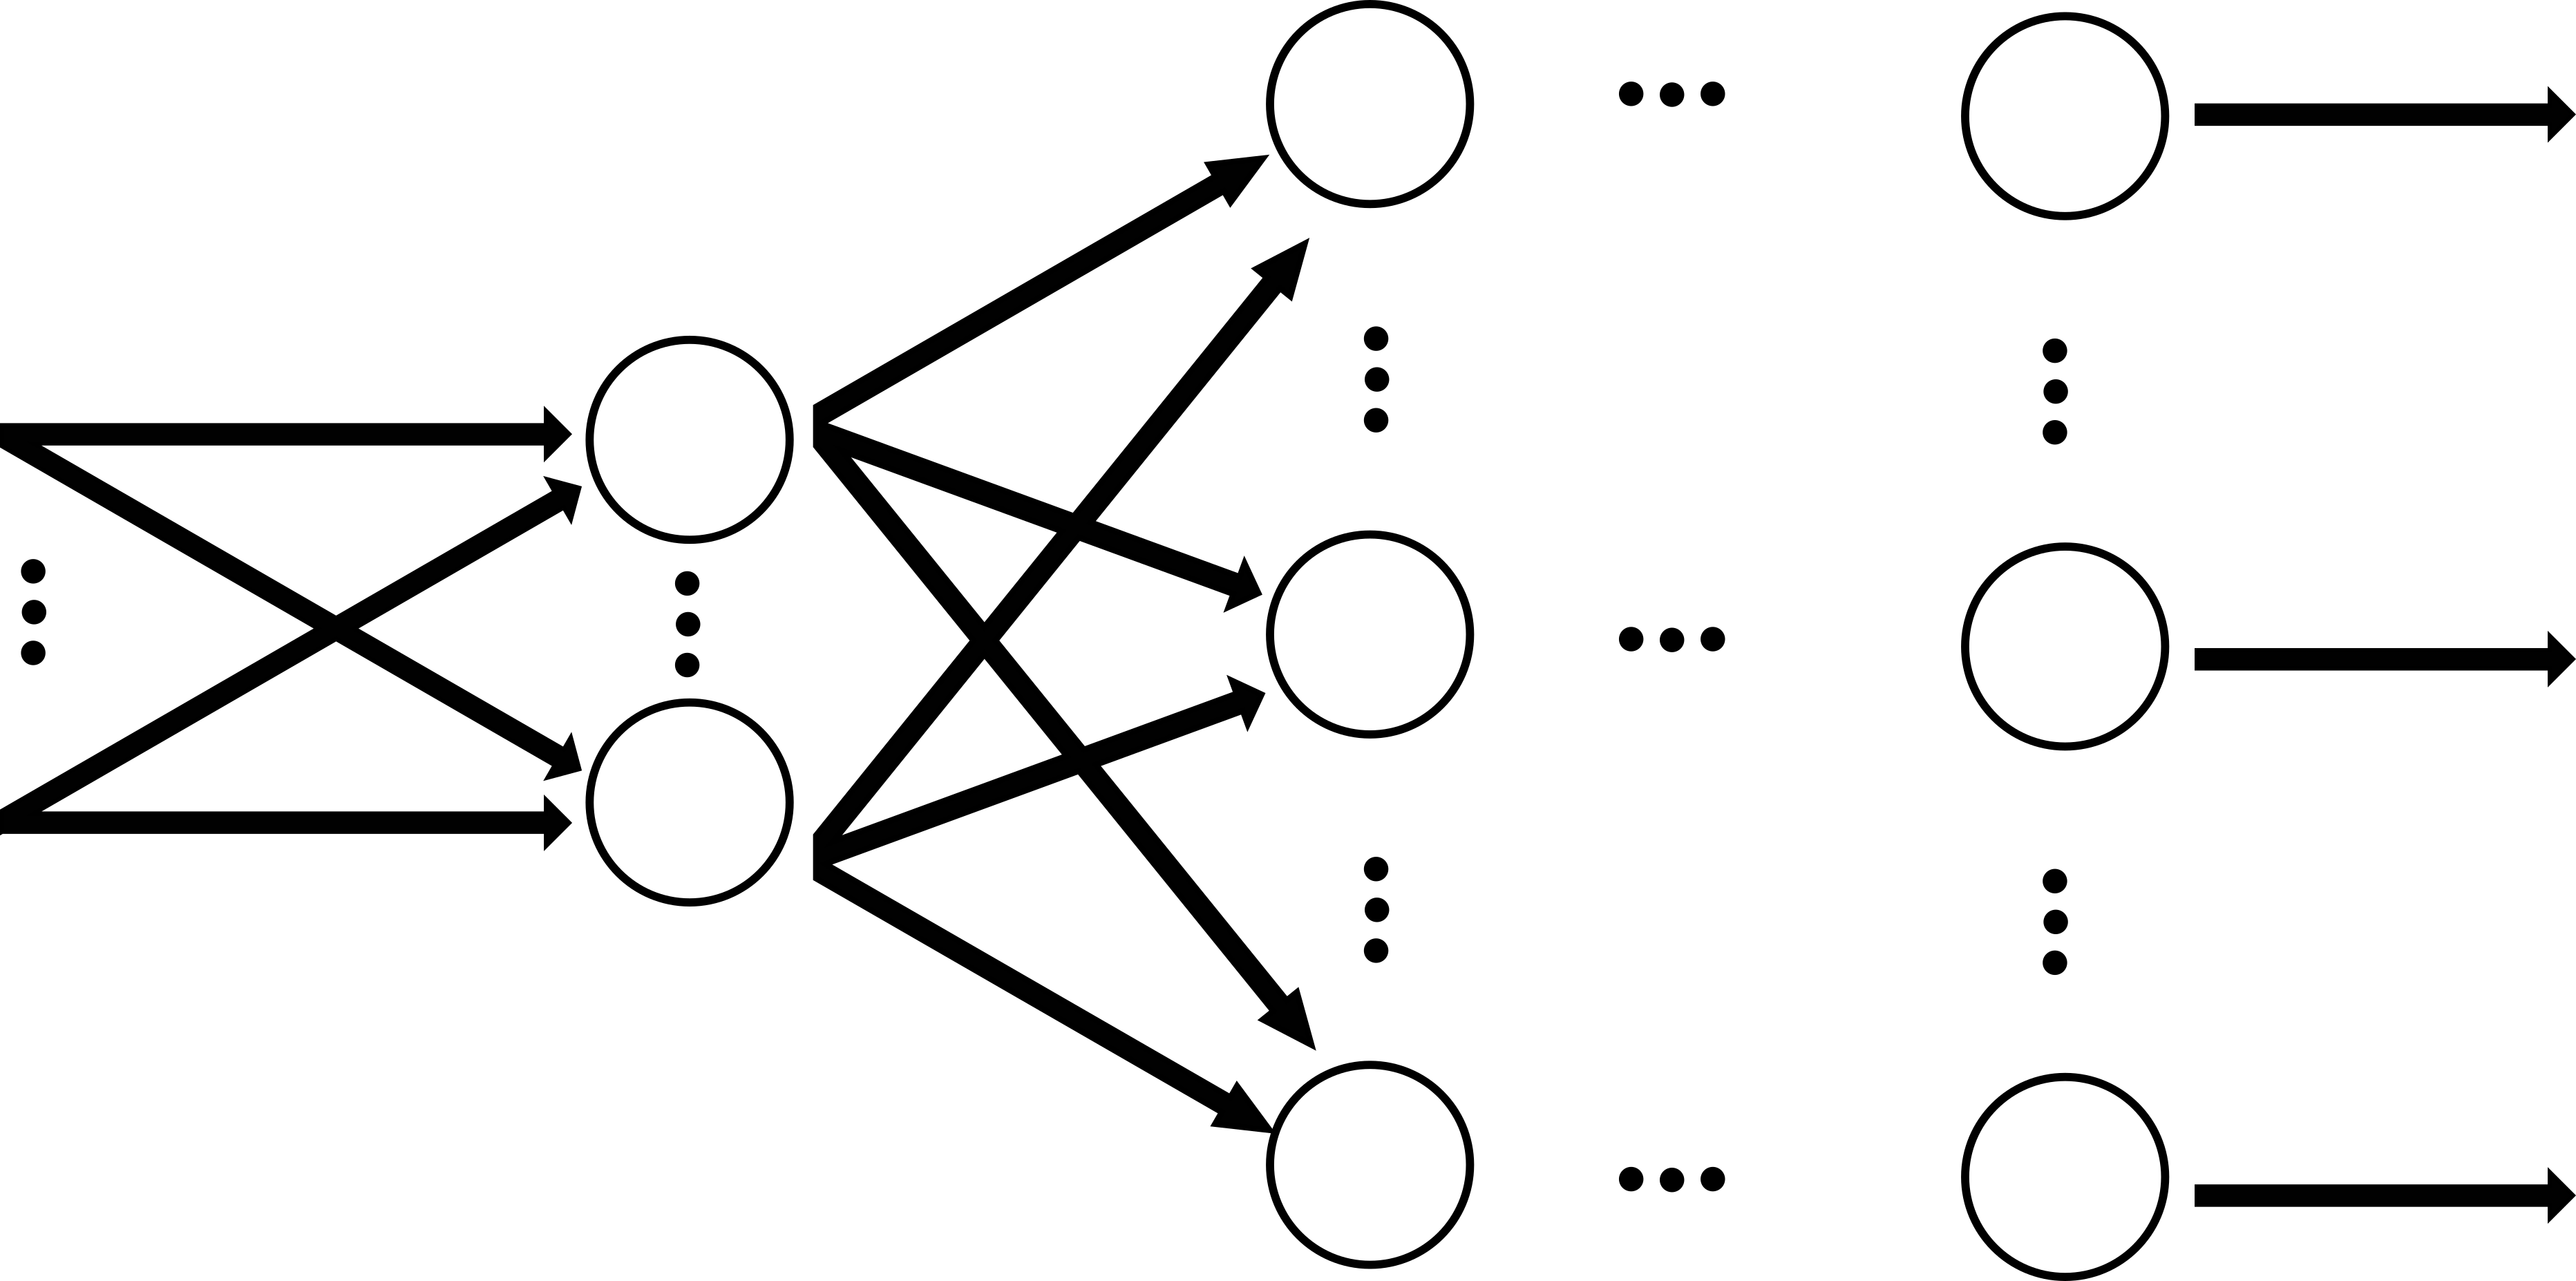
\includegraphics[height=50px]{2-Reseau.png}
  		\caption{Réseau de neurones}
	\end{subfigure}
	\begin{subfigure}[]{0.3\textwidth}
		\centering
		
\includegraphics[height=50px]{3-Matching.png}
		\caption{Correspondance phonétique}
	\end{subfigure}
\end{figure}
\end{frame}

% 1-INTRODUCTION
\section{I - Introduction}
\begin{frame}{I - Introduction}
\begin{block}{Présentation du modèle du Perceptron}
McCulloh et Pitts introduise le modèle du Perceptron en 1943, basé sur le fonctionnement du neurone humain.
\end{block}
\end{frame}

\begin{frame}{I - Introduction}
\begin{figure}
	\centering
    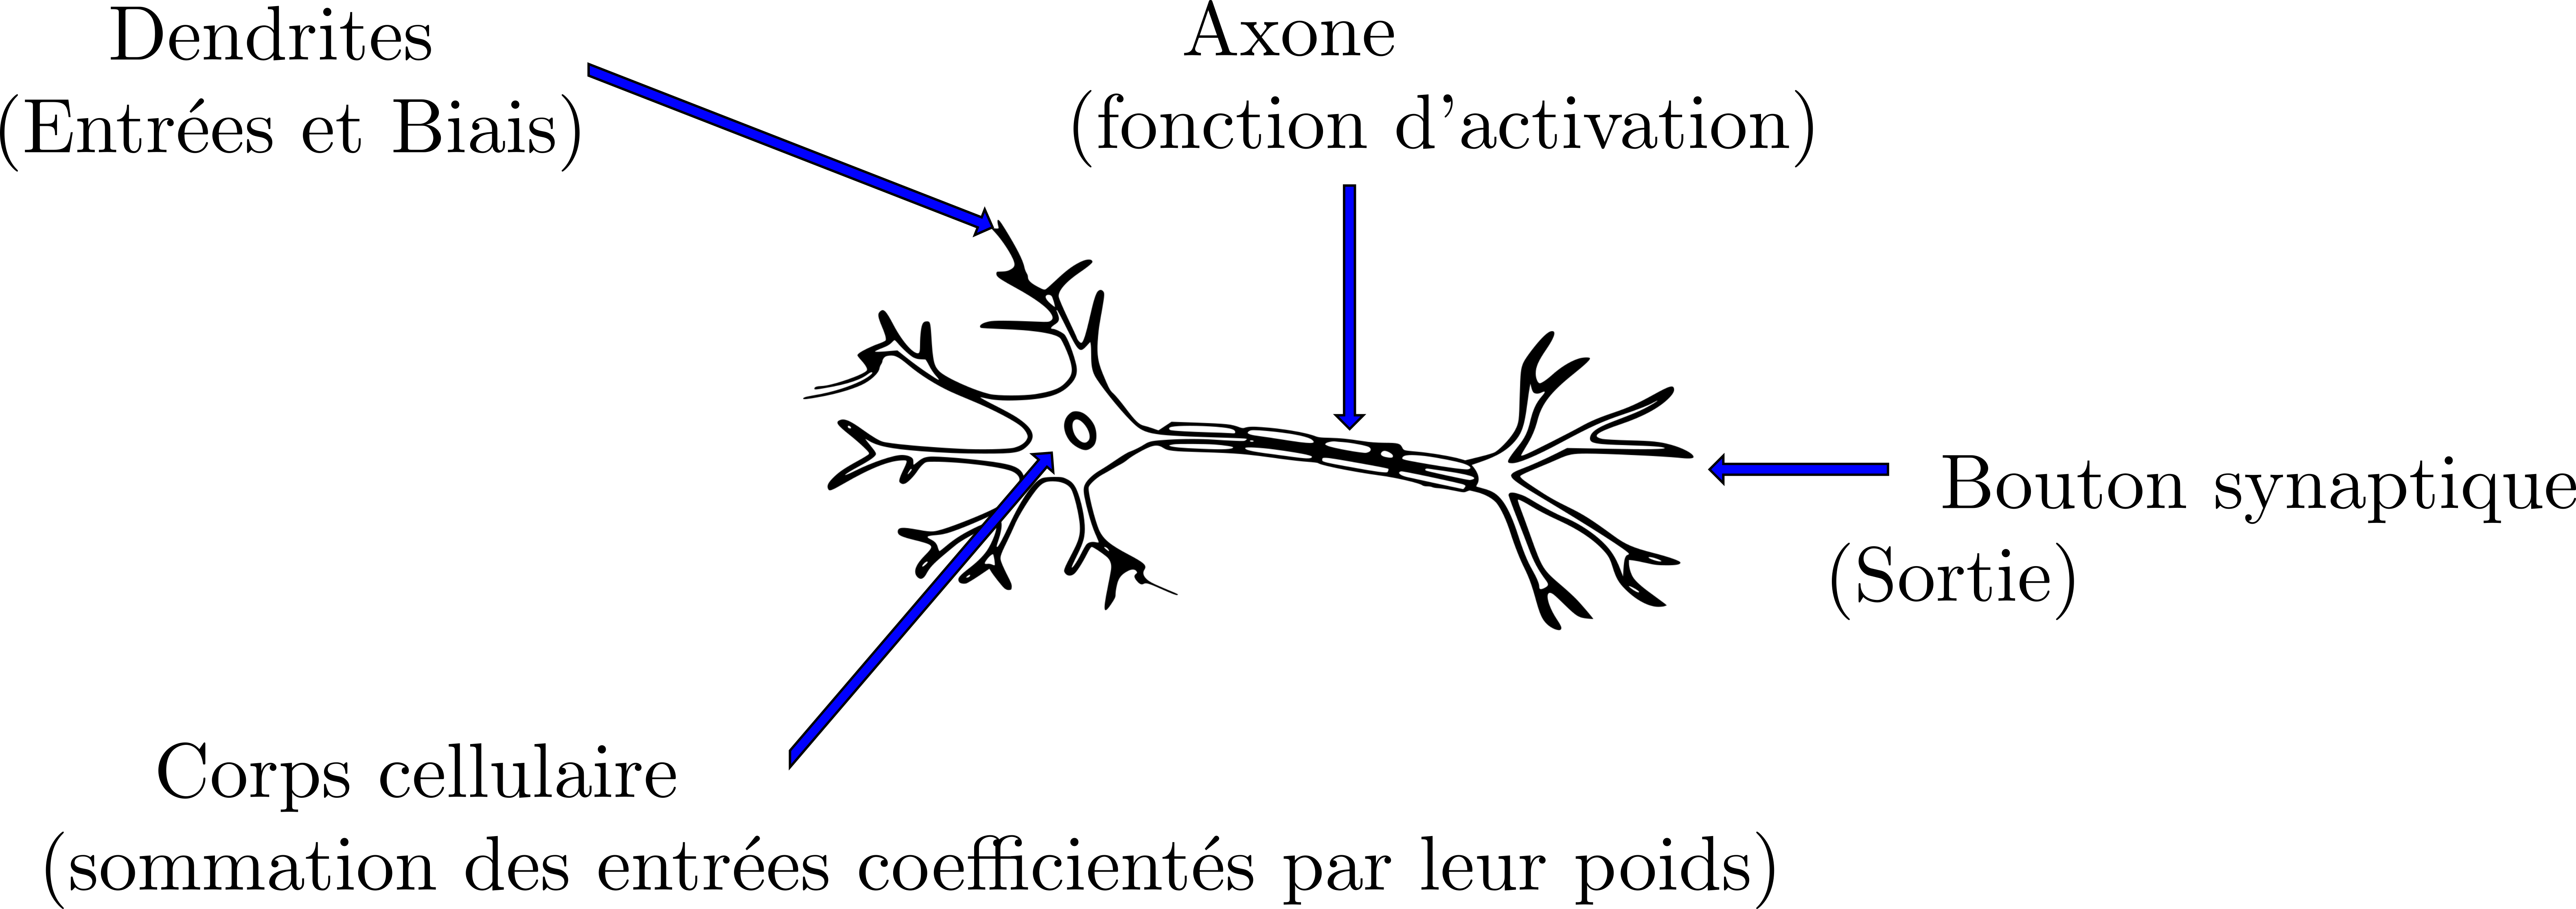
\includegraphics[height=75px]{2-Neurone.png}
	\caption{Schéma d'un neurone}	
\end{figure}
\begin{figure}
	\centering
    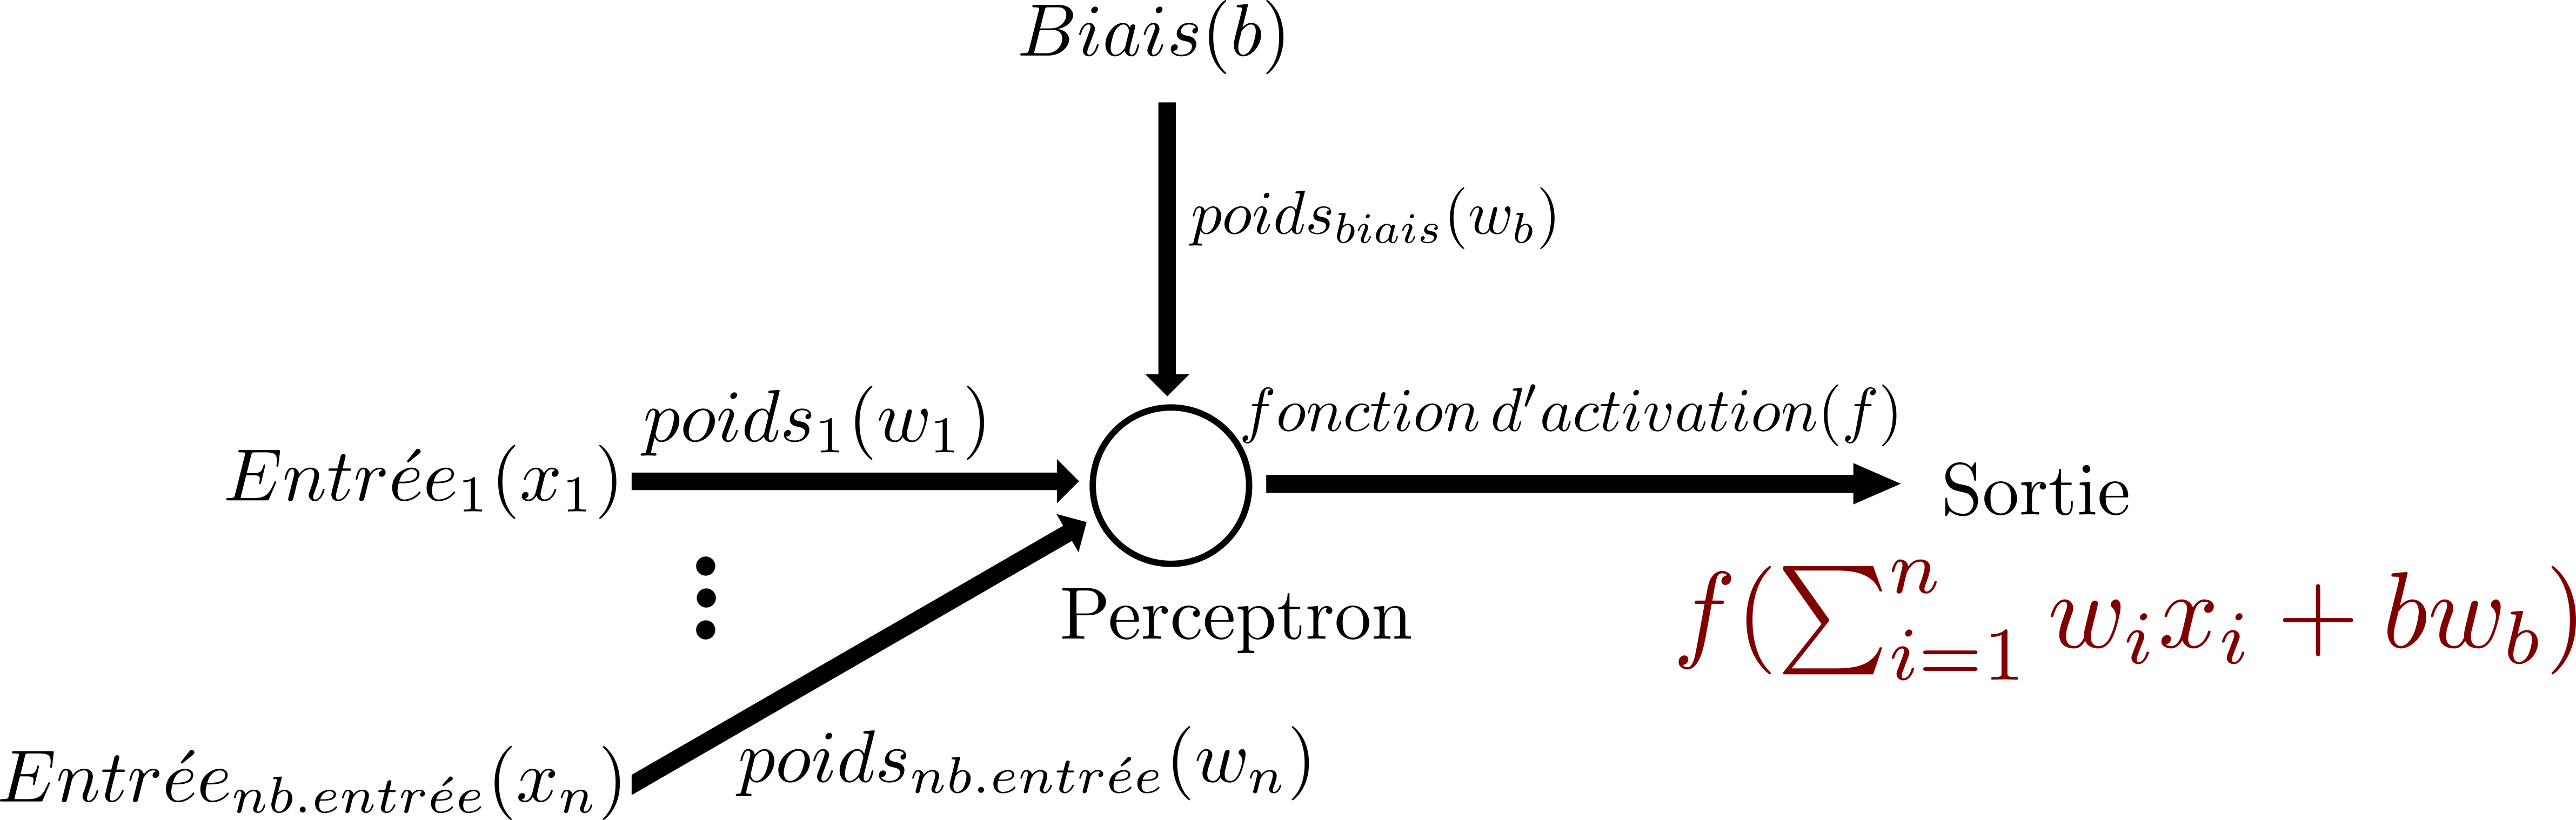
\includegraphics[height=75px]{1-Perceptron.png}
	\caption{Schéma d'un perceptron}	
\end{figure}
\end{frame}

% 2-Fonction d'activation
\section{II - Fonction d'activation}
\begin{frame}{II - Fonction d'activation}
\begin{block}{Fonction d'activation}
Sans l'utilisation de la fonction d'activation, le neurone est multilinéaire par rapport à ses entrées, il n'est donc capable que de faire des régressions linéaires sur les données d'entrées. \\
Les fonctions d'activation permettent donc une classification non linéaire.
\end{block}
\end{frame}


\begin{frame}{II - Représentation informatique}
\begin{figure}
	\centering
    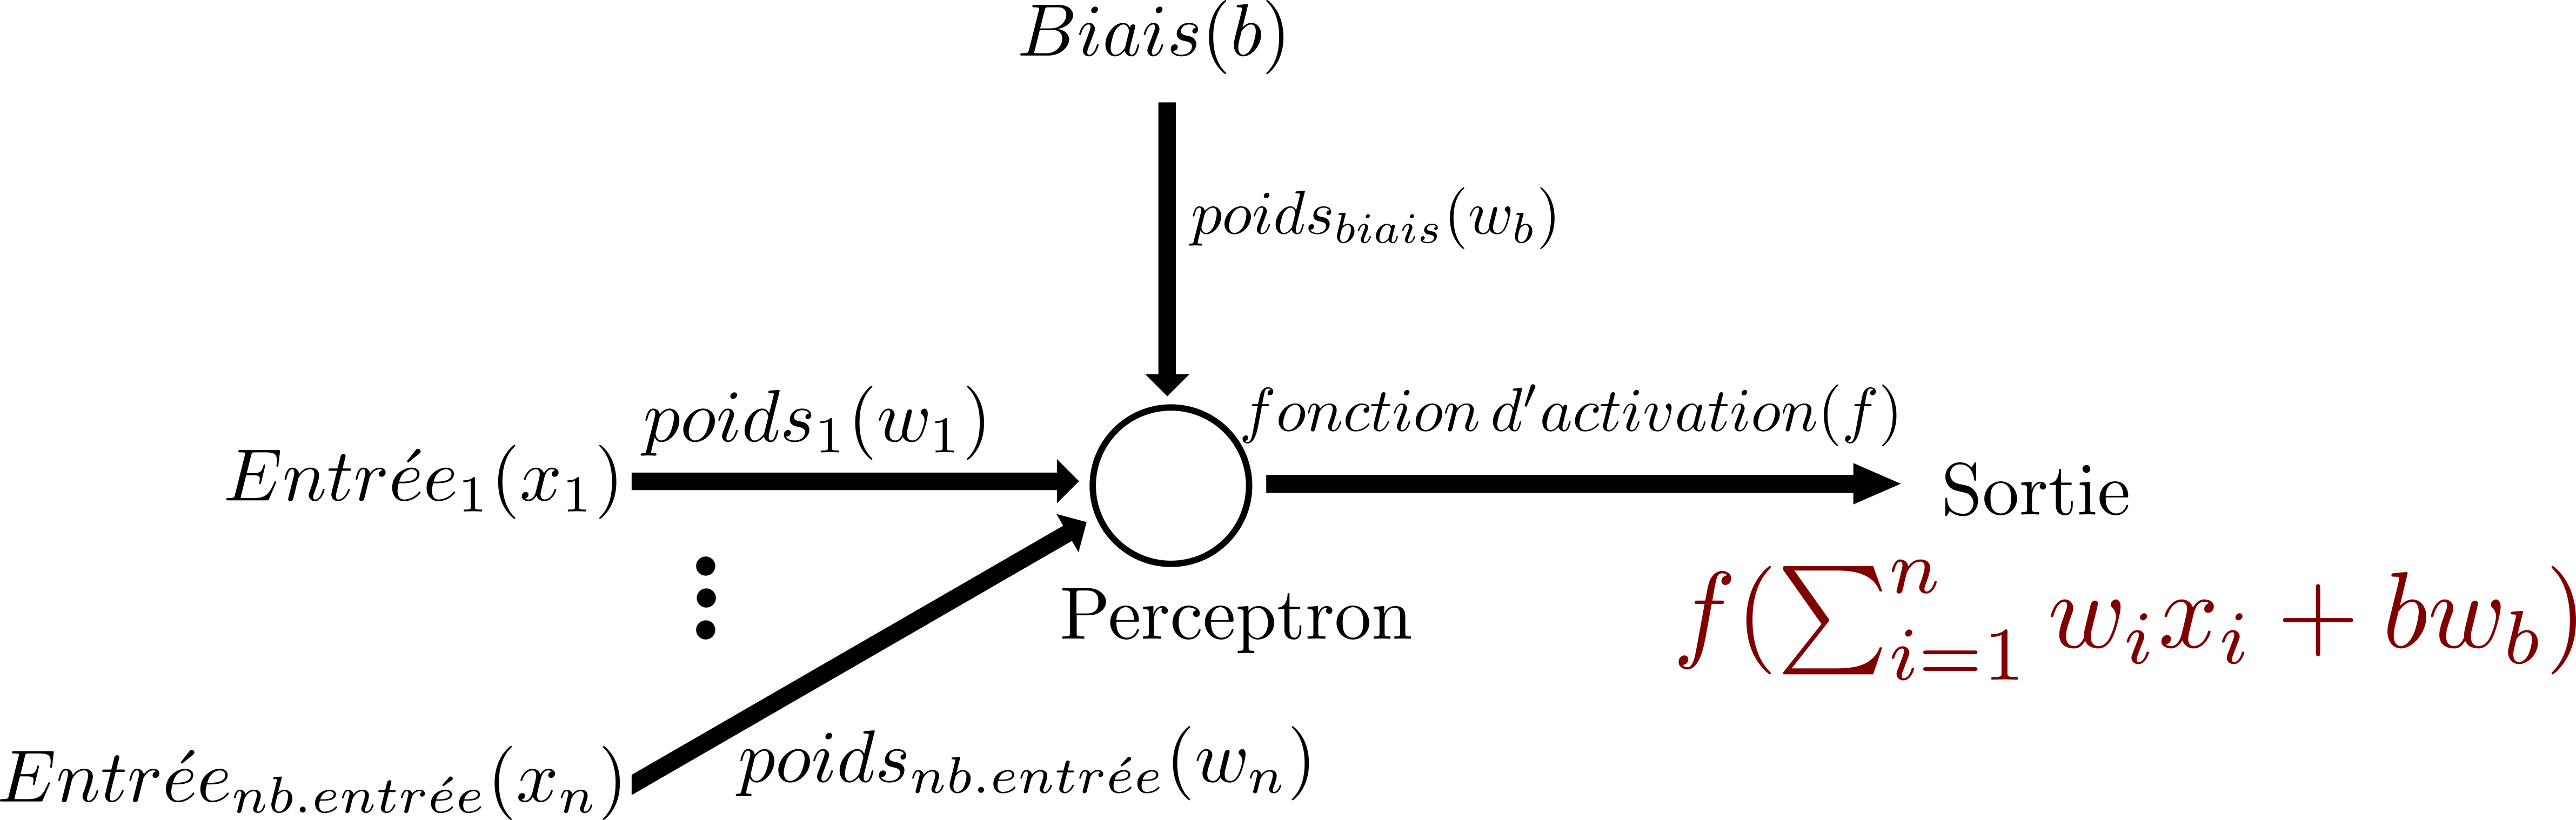
\includegraphics[height=75px]{1-Perceptron.png}
	\caption{Schéma d'un perceptron}	
\end{figure}
\begin{multicols}{2}
$
f
\left(
\begin{pmatrix}
x_1 & \ldots & x_n & b
\end{pmatrix}
\times
\begin{pmatrix}
w_1 \\
\vdots \\
w_n \\
w_b
\end{pmatrix}
\right)
$ \\
La complexité est en $O(n)$
\columnbreak
\lstinputlisting[language=Python]{code.py}
\end{multicols}
\end{frame}


\begin{frame}{II - Fonction d'activation}
\begin{figure}
	\begin{subfigure}[]{0.3\textwidth}
		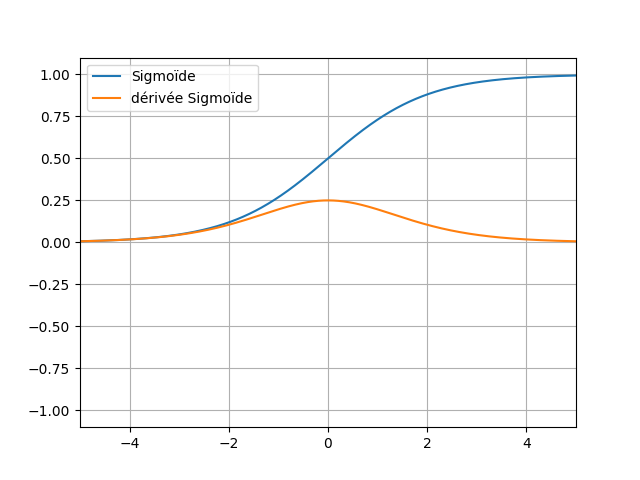
\includegraphics[width=90px]{0-Sigmoide.png}
  		\caption{Sigmoïde}
	\end{subfigure}
	\begin{subfigure}[]{0.3\textwidth}
		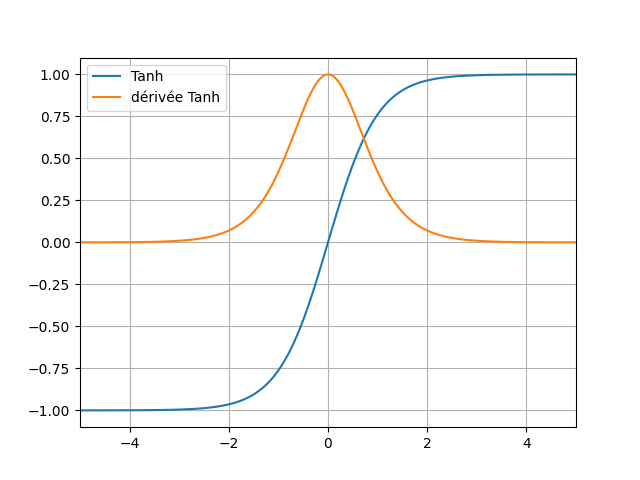
\includegraphics[width=90px]{0-Tanh.png}
  		\caption{Tanh}
	\end{subfigure}
	\begin{subfigure}[]{0.3\textwidth}
		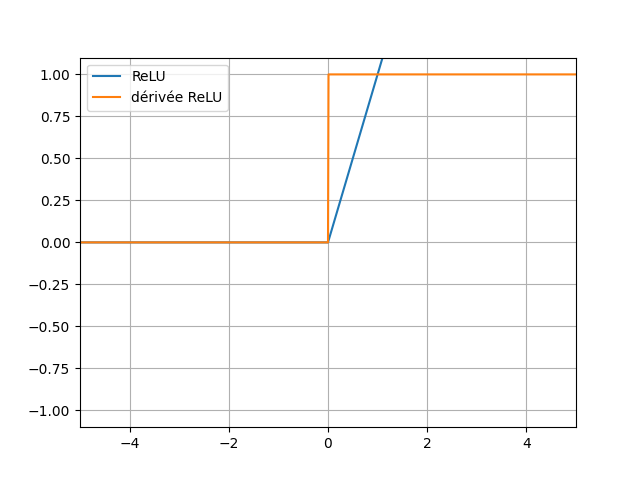
\includegraphics[width=90px]{0-ReLU.png}
		\caption{ReLU}
	\end{subfigure}
\end{figure}

\begin{block}{}
\centering
\begin{tabular}{ l || c | c | }
   Fonction & Formule & Dérivée \\ \hline \\
   Sigmoïde (a) & $\mathlarger{\frac{1}{1+e^{-x}}}$ & $f(x) \times (1-f(x))$ \\ \\
   Tangente Hyperbolique (Tanh) (b) & $\mathlarger{\frac{e^{x}-e^{-x}}{e^{x}-e^{-x}}}$ & $1-f(x)^2$ \\ \\
   Unité Linéaire Rectifiée (ReLU) (c) & $max(0, x)$ & $ \left\{\begin{array}{ll}
      														  0 & \mbox{si } x<0 \\
     														  1 & \mbox{sinon }   \end{array}\right.$ \\
\end{tabular}
\end{block}
\end{frame}

\begin{frame}{II - Fonction d'activation, les spécificités}


\begin{block}{}
\centering
\begin{tabular}{ |p{0.15\textwidth}||p{0.35\textwidth}|p{0.35\textwidth} | }
\hline 
   Fonction & Avantage & Inconvénient \\ [20pt] \hline \hline 
   Sigmoïde & A valeur dans ]0, 1[ ce qui facilite les classifications binaires & Dérivée petite vers $\pm\infty$, il y a peu d'apprentissage pour ces valeurs \\ [20pt] \hline
   Tanh & Utilisé dans les couches cachées car fonction impaire  & Même problème que la Sigmoïde \\ [20pt] \hline
   ReLU & Plus simple à calculer, prend en compte le grandient pour toute valeur positive & Dérivée nulle en x négatif ce qui peut rendre des neurones inutiles \\ [20pt] \hline 
\end{tabular}
\end{block}
\end{frame}


% 3-Descente de gradient
\section{III - Descente de gradient}
\begin{frame}{Descente de gradient}
\begin{block}{Descente de gradient}
La Descente de Gradient est un algorithme d’optimisation qui permet de trouver un minimum local d'une fonction en convergeant progressivement. \\
Dans l'apprentissage des réseaux de neurones, la descente de gradient est utilisée pour trouver le minimum d'une fonction coût, évaluant l'erreur entre la valeur de sortie du réseau et celle attendu. \\
La fonction d'erreur est noté $f : s \mapsto (s - s_{attendue})^2$, avec $s$ la sortie donnée par le modèle et $s_{attendue}$ la sortie cible. \\
En effet, trouver des paramètres (poids, architecture du réseau, fonction d'activation) permettant d'avoir une erreur nulle revient à résoudre le problème qu'évalue cette fonction coût par rapport aux entrées données.
\end{block}
\end{frame}

\begin{frame}{III - Descente de gradient}
\begin{block}{Algorithme du gradient}
Soit $n \in \mathbb{N}, \varepsilon > 0$. On munit $\mathbb{R}^n$ de son produit scalaire canonique. \newline
    Soit $f$ une fonction différentiable de $\mathbb{R}^n \to \mathbb{R}$. \newline
    Soit $x_0$ une valeur initiale aléatoire, $t$ le taux d'apprentissage. \newline
    Supposons $x_0, \ldots, x_k$ construits. \newline
    • Si $\norme{\nabla f(x_k)} \leq \varepsilon$, on s'arrête. \newline
    • Sinon on pose $x_{k+1} = x_k - t \nabla f(x_k)$ \newline
\end{block}

\begin{figure}
	\centering
    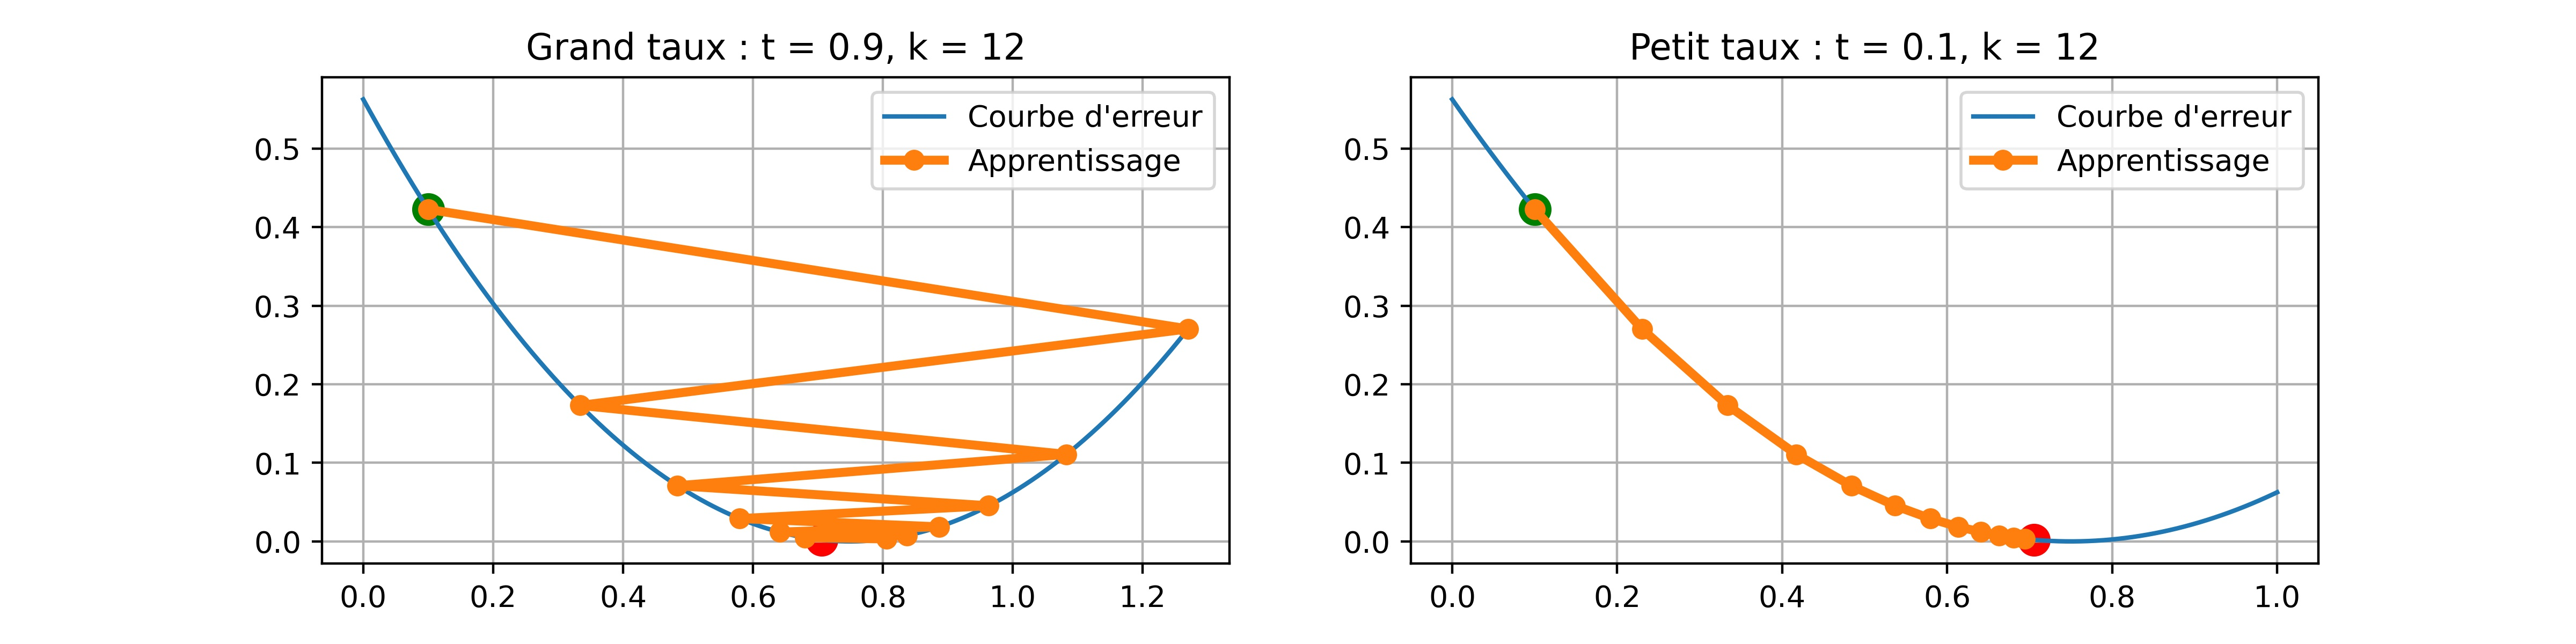
\includegraphics[height=75px]{1-DescenteGradient.jpg}
	\caption{Descente de Gradient pour $f(x) = (x-0.75)^2$; $x_0=0.1$ et $\varepsilon = 0.1$}
\end{figure}
\end{frame}

\begin{frame}{III - Importance du choix du taux d'apprentissage}
Pour la suite on continuera avec la fonction $f(x) = (x-0.75)^2$ et $x_0=0.1$. \\
On montre qu'en choisissant un taux d'apprentissage trop petit ou trop grand, il est possible que la descente de gradient diverge, ou ne converge pas assez vite.
\begin{figure}
	\centering
    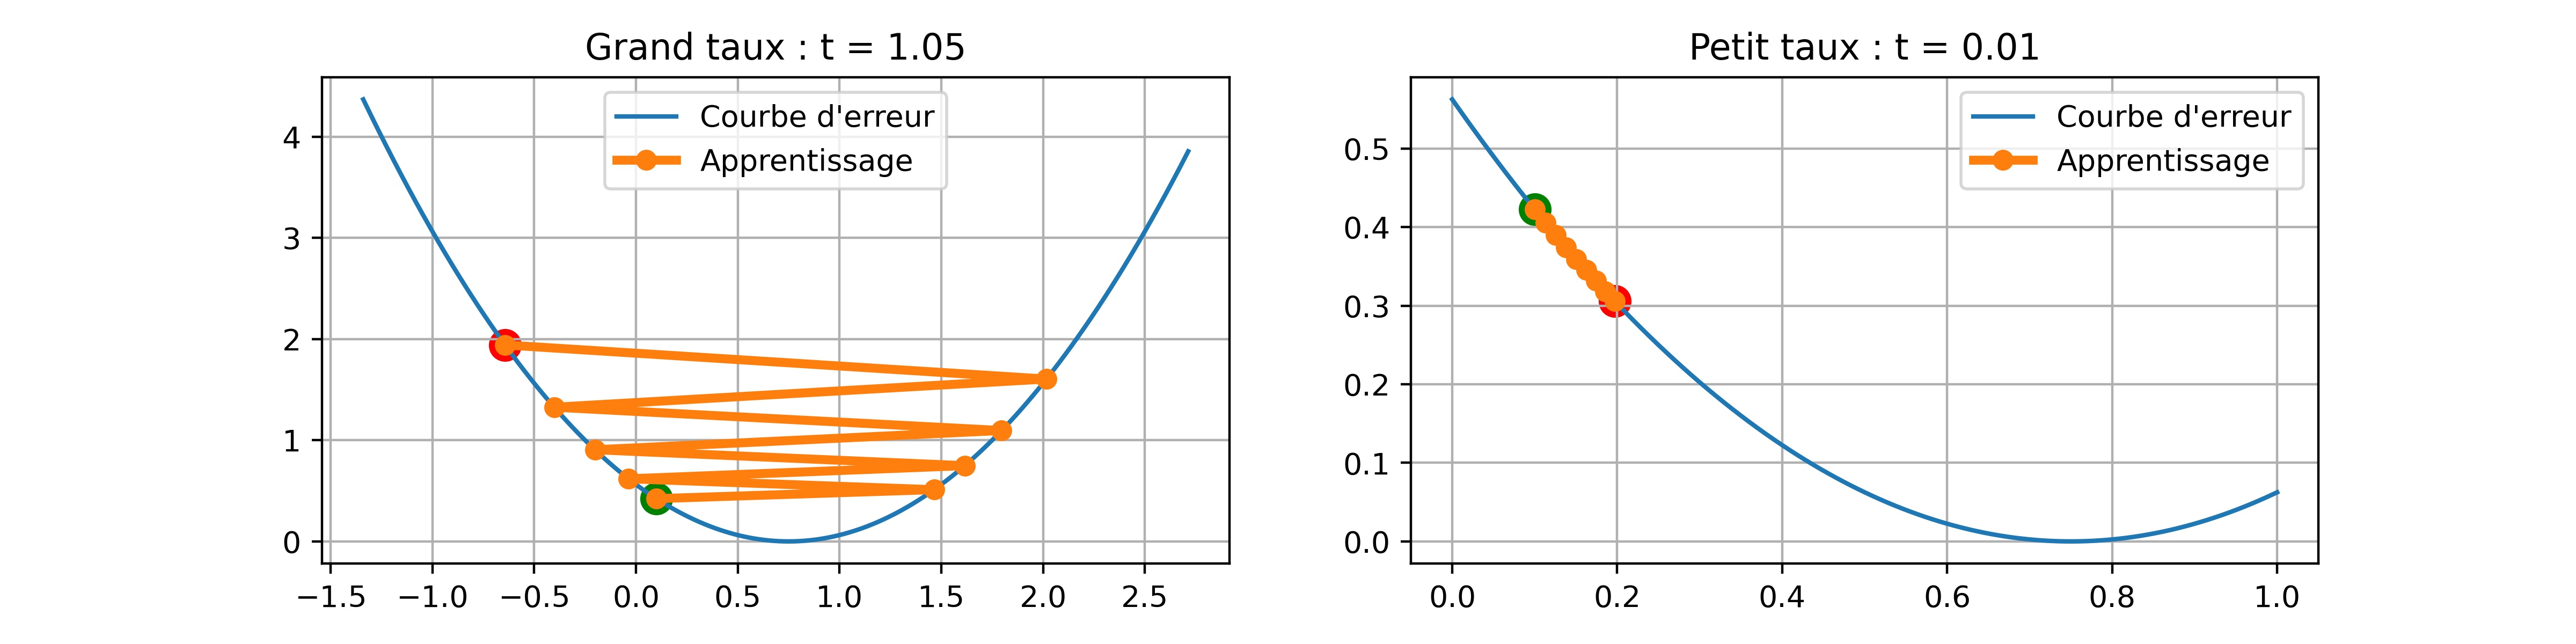
\includegraphics[height=80px]{2-DescenteGradient.jpg}
	\caption{Descente de Gradient on force l'arrêt à $k=8$}
\end{figure}
\end{frame}

\begin{frame}{III - Utilisation du Moment}
\begin{block}{III - Descente de gradient avec moment}
$x_0$ aléatoire et le moment $\omega_0 = 0$.
Supposons $x_0, \ldots, x_k$ et $\omega_0, \ldots, \omega_k$ construits. \\
    • On pose $\omega_{k+1} = \gamma \omega_k + t \nabla f(x_k)$ \\
    • On pose $x_{k+1} = x_k - \omega_{k+1}$ 
\end{block}
\begin{figure}
	\centering
    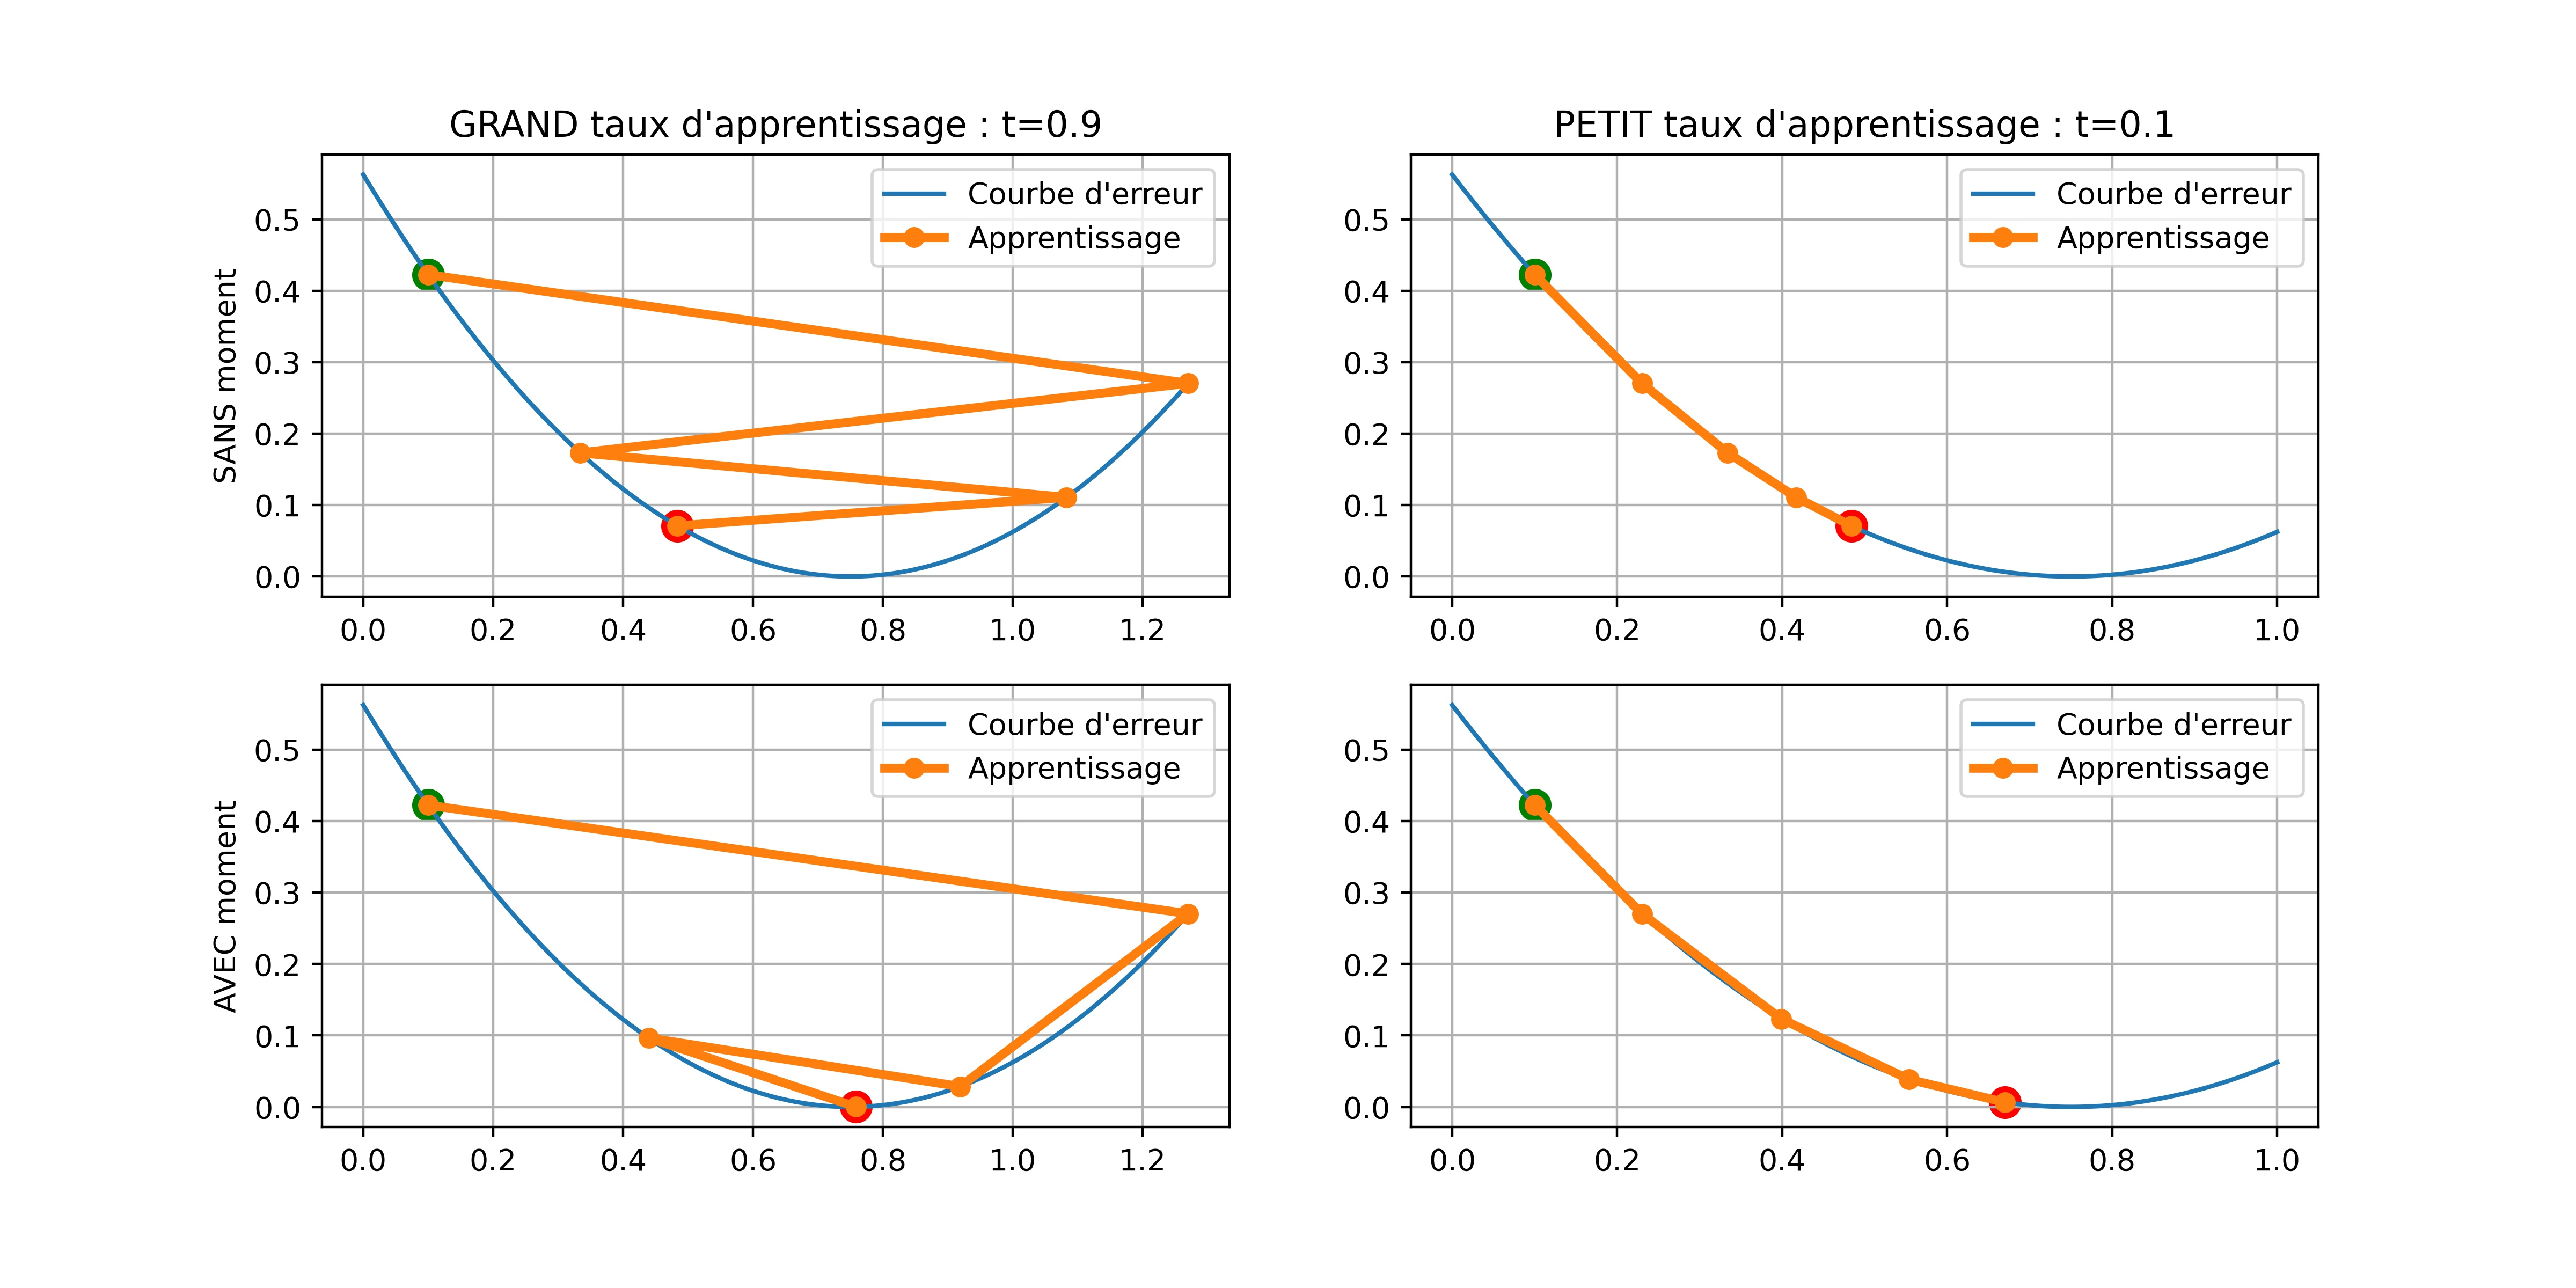
\includegraphics[height=130px, trim=0 35 0 35, clip]{3-Moment.jpg}
	\caption{Comparaison sans puis avec dépendance au moment avec $\gamma = 0.5$, arrêt à $k=4$}
\end{figure}
\end{frame}

\begin{frame}{III - Utilisation du Moment}
Voici, une simulation pour des taux d'apprentissage "trop grand" ou "trop petit".
\begin{figure}
	\centering
    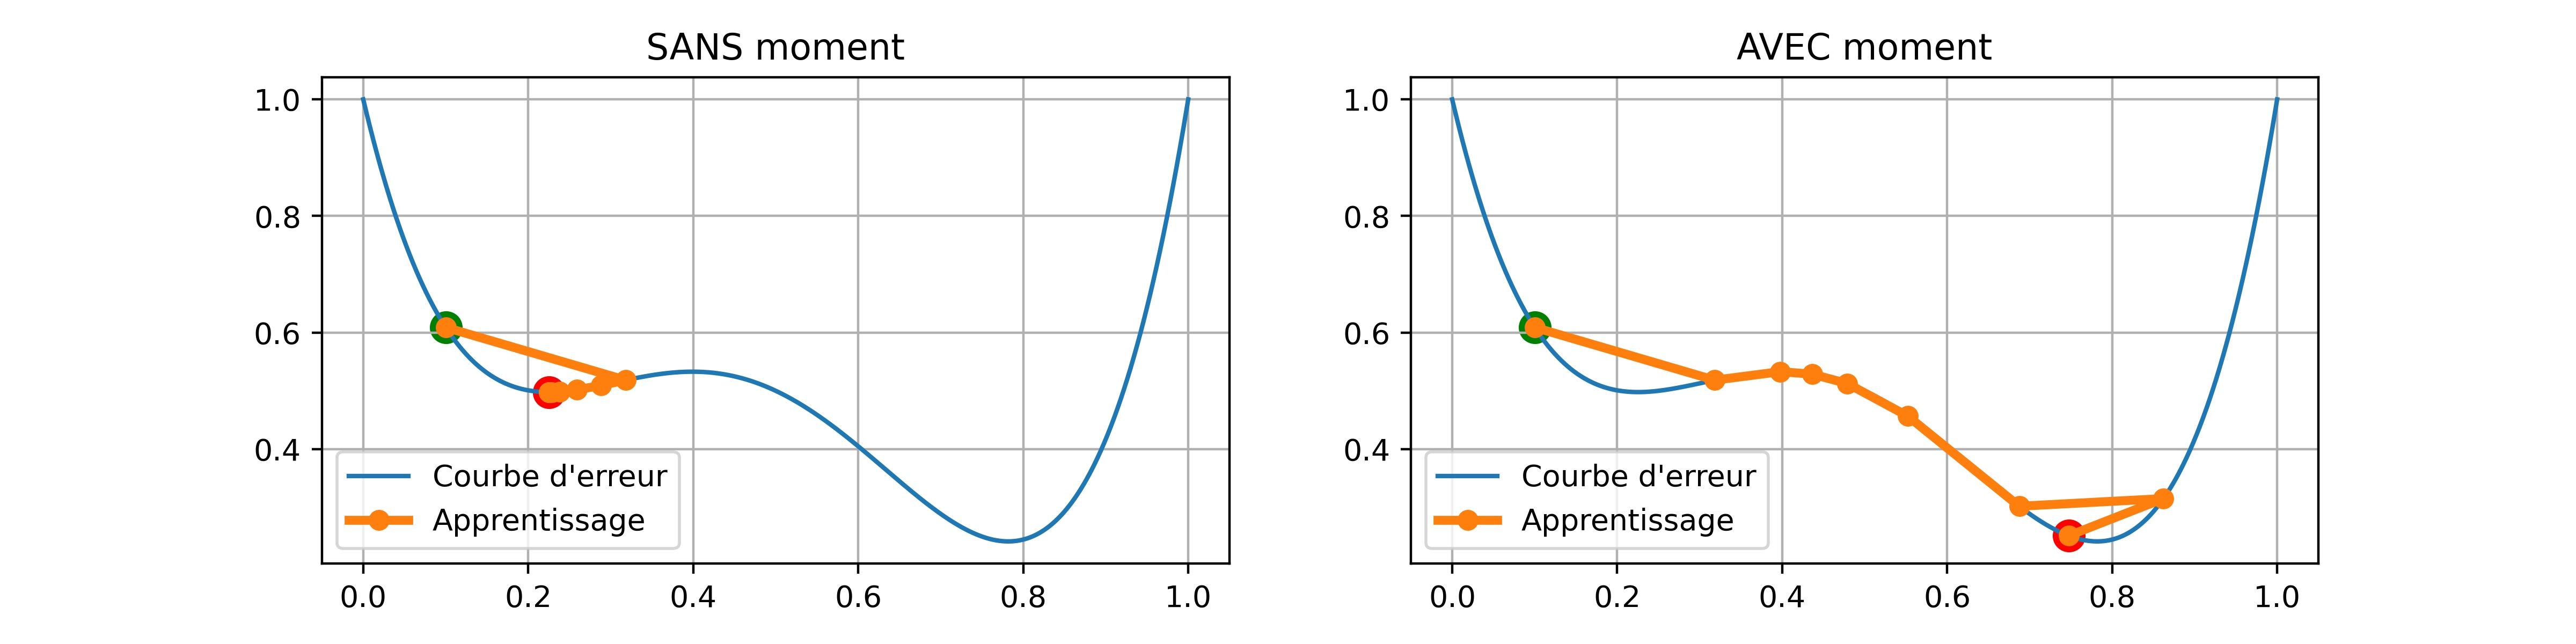
\includegraphics[height=130px, trim=0 35 0 35, clip]{4-Moment.jpg}
	\caption{Comparaison sans puis avec dépendance au moment avec $\gamma = 0.5$, arrêt à $k=8$}
\end{figure}
\end{frame}

\begin{frame}{III - Utilisation du Moment}
Le moment permet également de s'échapper de certain minimum locaux.
\begin{figure}
	\centering
    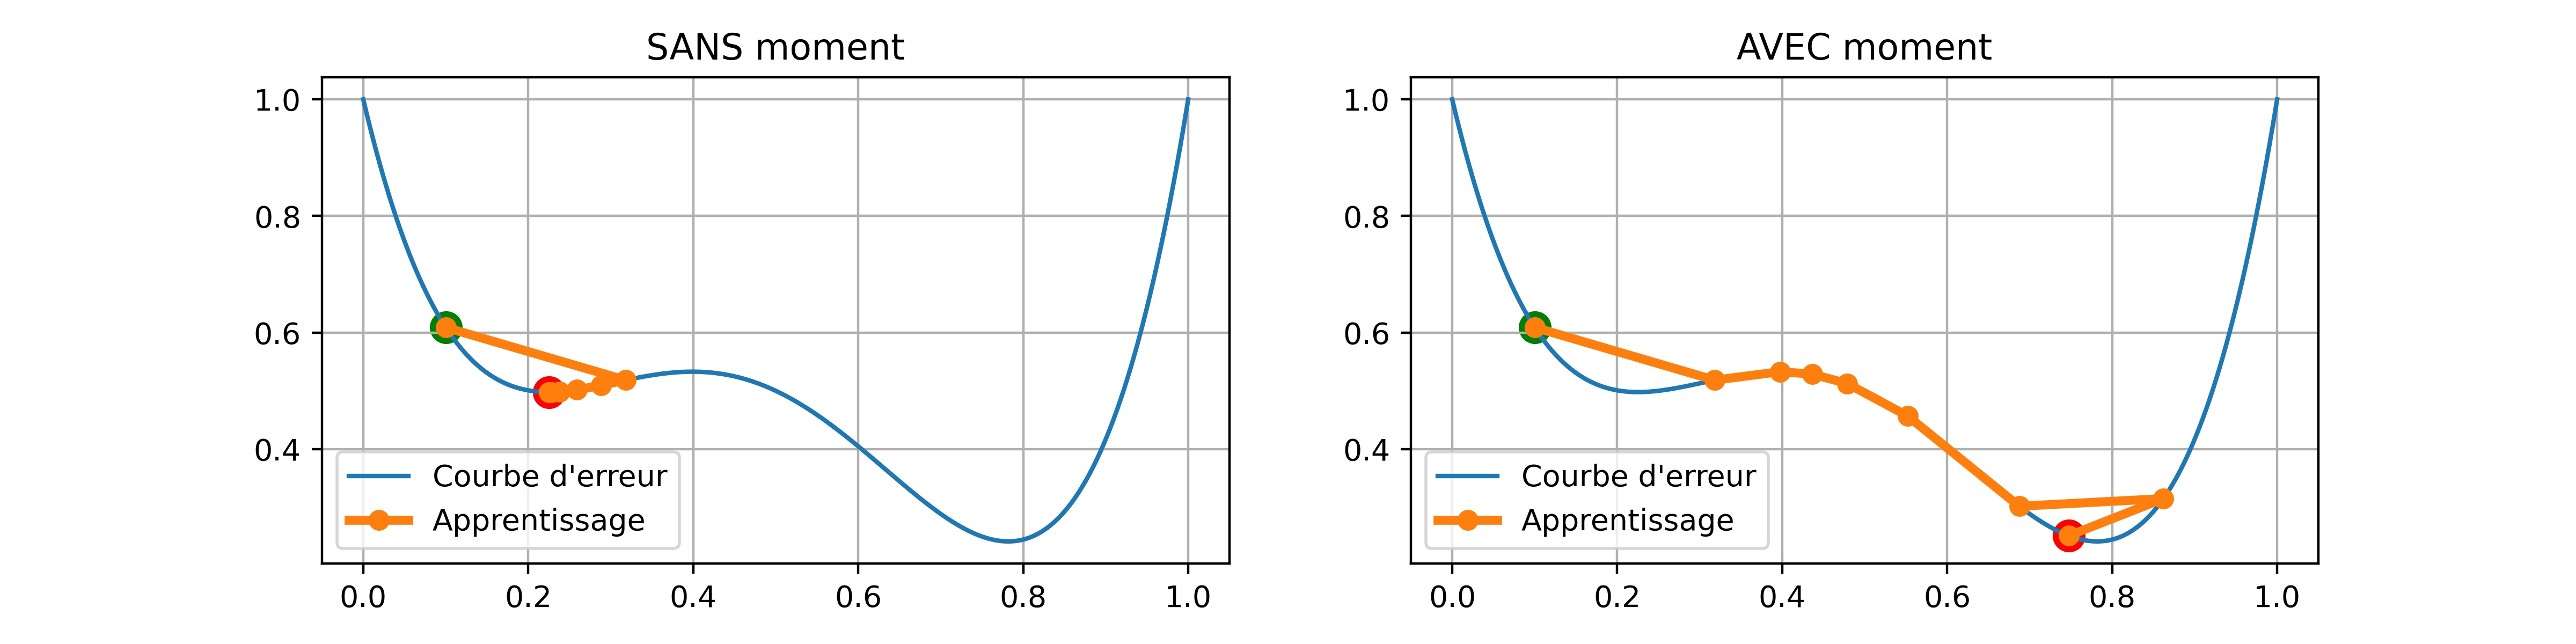
\includegraphics[width=\textwidth, trim=0 10 0 10, clip]{5-Moment.jpg}
	\caption{Comparaison sans puis avec dépendance au moment avec $\gamma = 0.5$, arrêt à $k=8$}
\end{figure}
\end{frame}

\begin{frame}{III - Apprentissage stochastique ou par paquet (Batch)}
Les paramètres du réseau de neurone sont les poids qui pondèrent l'entrée. C'est sur eux que l'on opèrent la descente de gradient. 
\begin{figure}
	\centering
    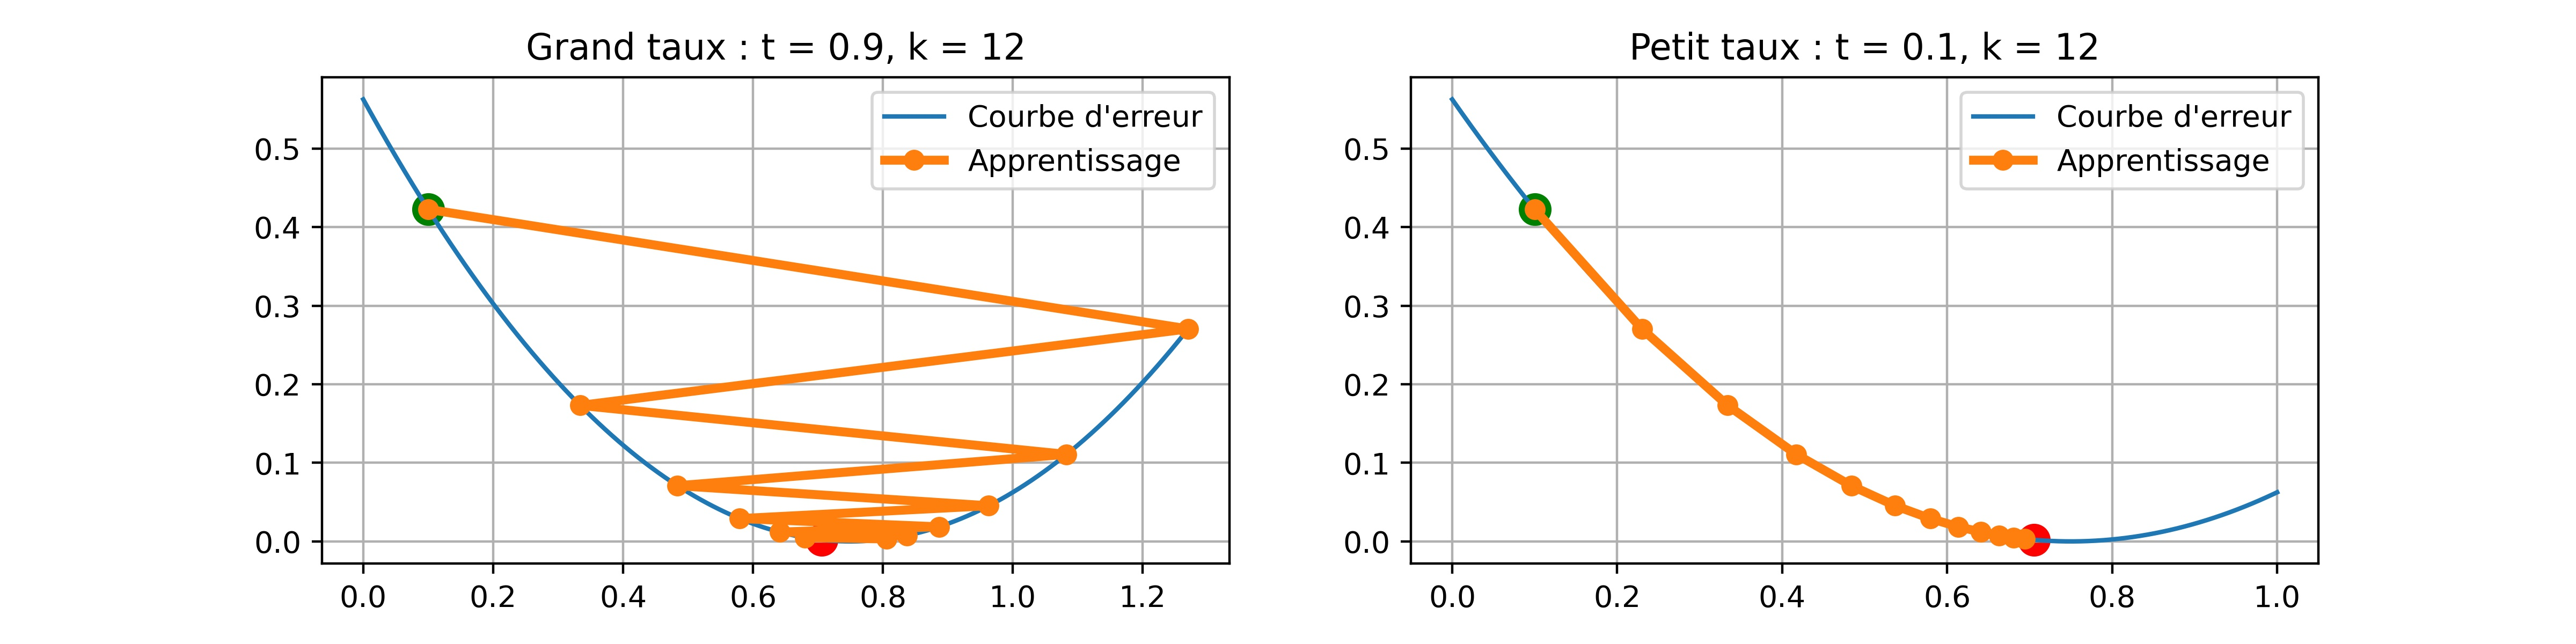
\includegraphics[width=\textwidth]{1-DescenteGradient.jpg}
\end{figure}
\begin{figure}
	\centering
    
\includegraphics[height=50px]{6-Perceptron.png}
	\caption{Schéma du perceptron linéaire}
\end{figure}
\end{frame}

\begin{frame}{III - Apprentissage stochastique ou par paquet (Batch)}
\begin{multicols}{2}
Il faut prendre en compte le fait que les D données d'apprentissage ne sont pas toujours exactes, elles sont forcément inscrites dans une marge d'erreur. 
\columnbreak
$
\left< f
\left(
\begin{pmatrix}
x_1^{1} & \ldots & x_n^{1} & b \\
\vdots & \vdots & \vdots & \vdots \\
x_1^{D} & \ldots & x_n^{D} & b
\end{pmatrix}
\times
\begin{pmatrix}
w_1 \\
\vdots \\
w_n \\
w_b
\end{pmatrix}
\right) \right>
$
\end{multicols}
\begin{figure}
	\centering
    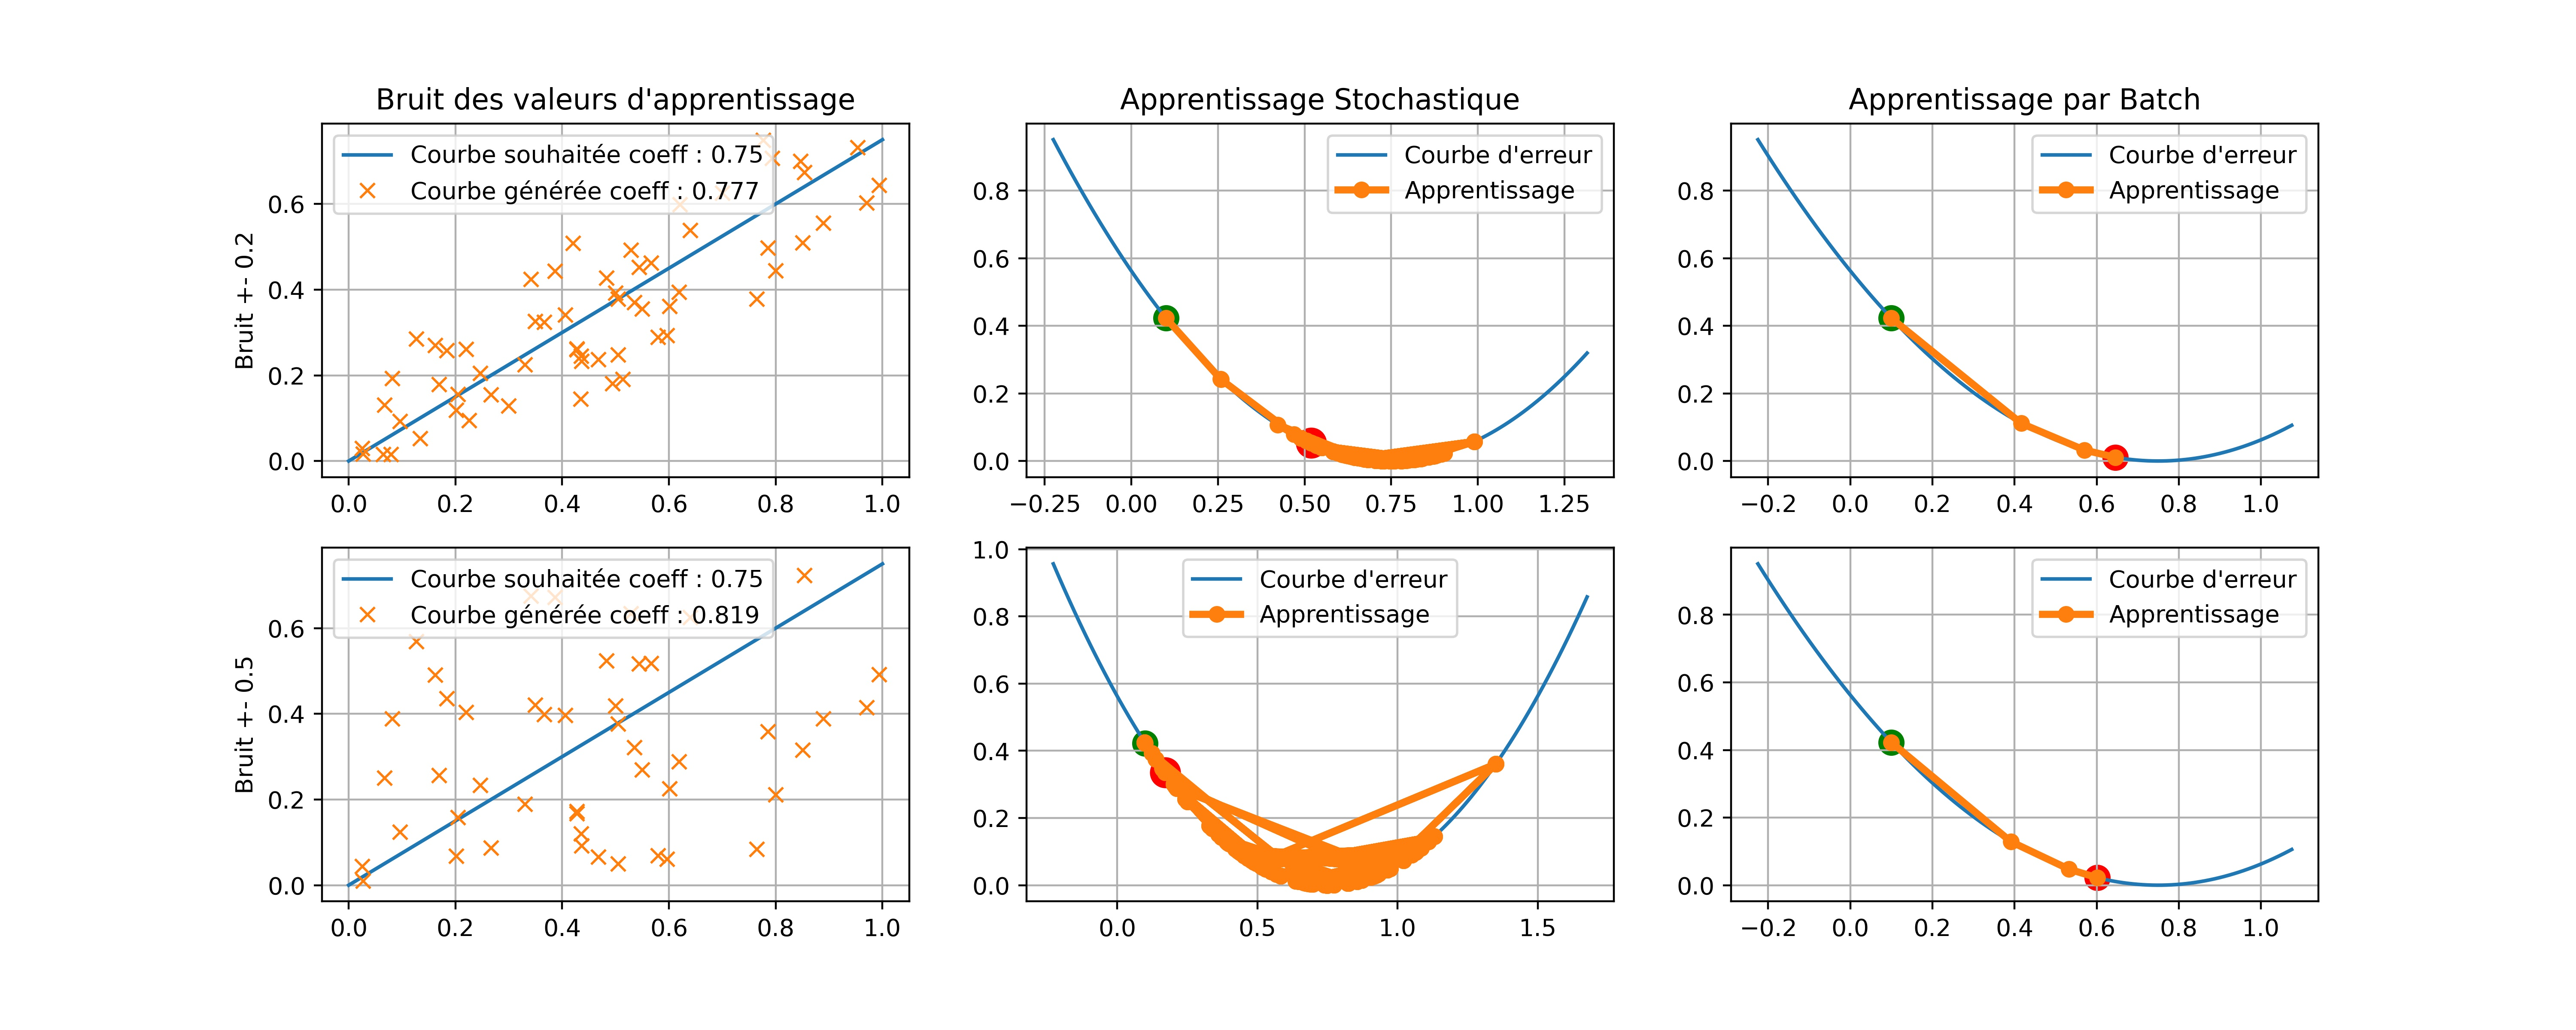
\includegraphics[width=\textwidth, trim=0 30 0 30, clip]{7-Batch.jpg}
	\caption{Comparaison apprentissage stochastique et par paquet, $f(x) = (x-0.75)^2$}
\end{figure}
\end{frame}

% 4-Problème de reproduction de l'opérateur XOR
\section{IV - Problème de reproduction de l'opérateur XOR}
\begin{frame}{IV - Problème de reproduction de l'opérateur XOR}
\begin{block}{Problème non linéairement séparables}
Un perceptron ou une couche de perceptron est incapable de reproduire des opérateurs non linéairement séparables. \\
Il faut alors mettre les perceptrons en série, pour former des couches cachées, pour pouvoir reproduire ces opérateurs. \\
\end{block}
\begin{figure}
	\centering
    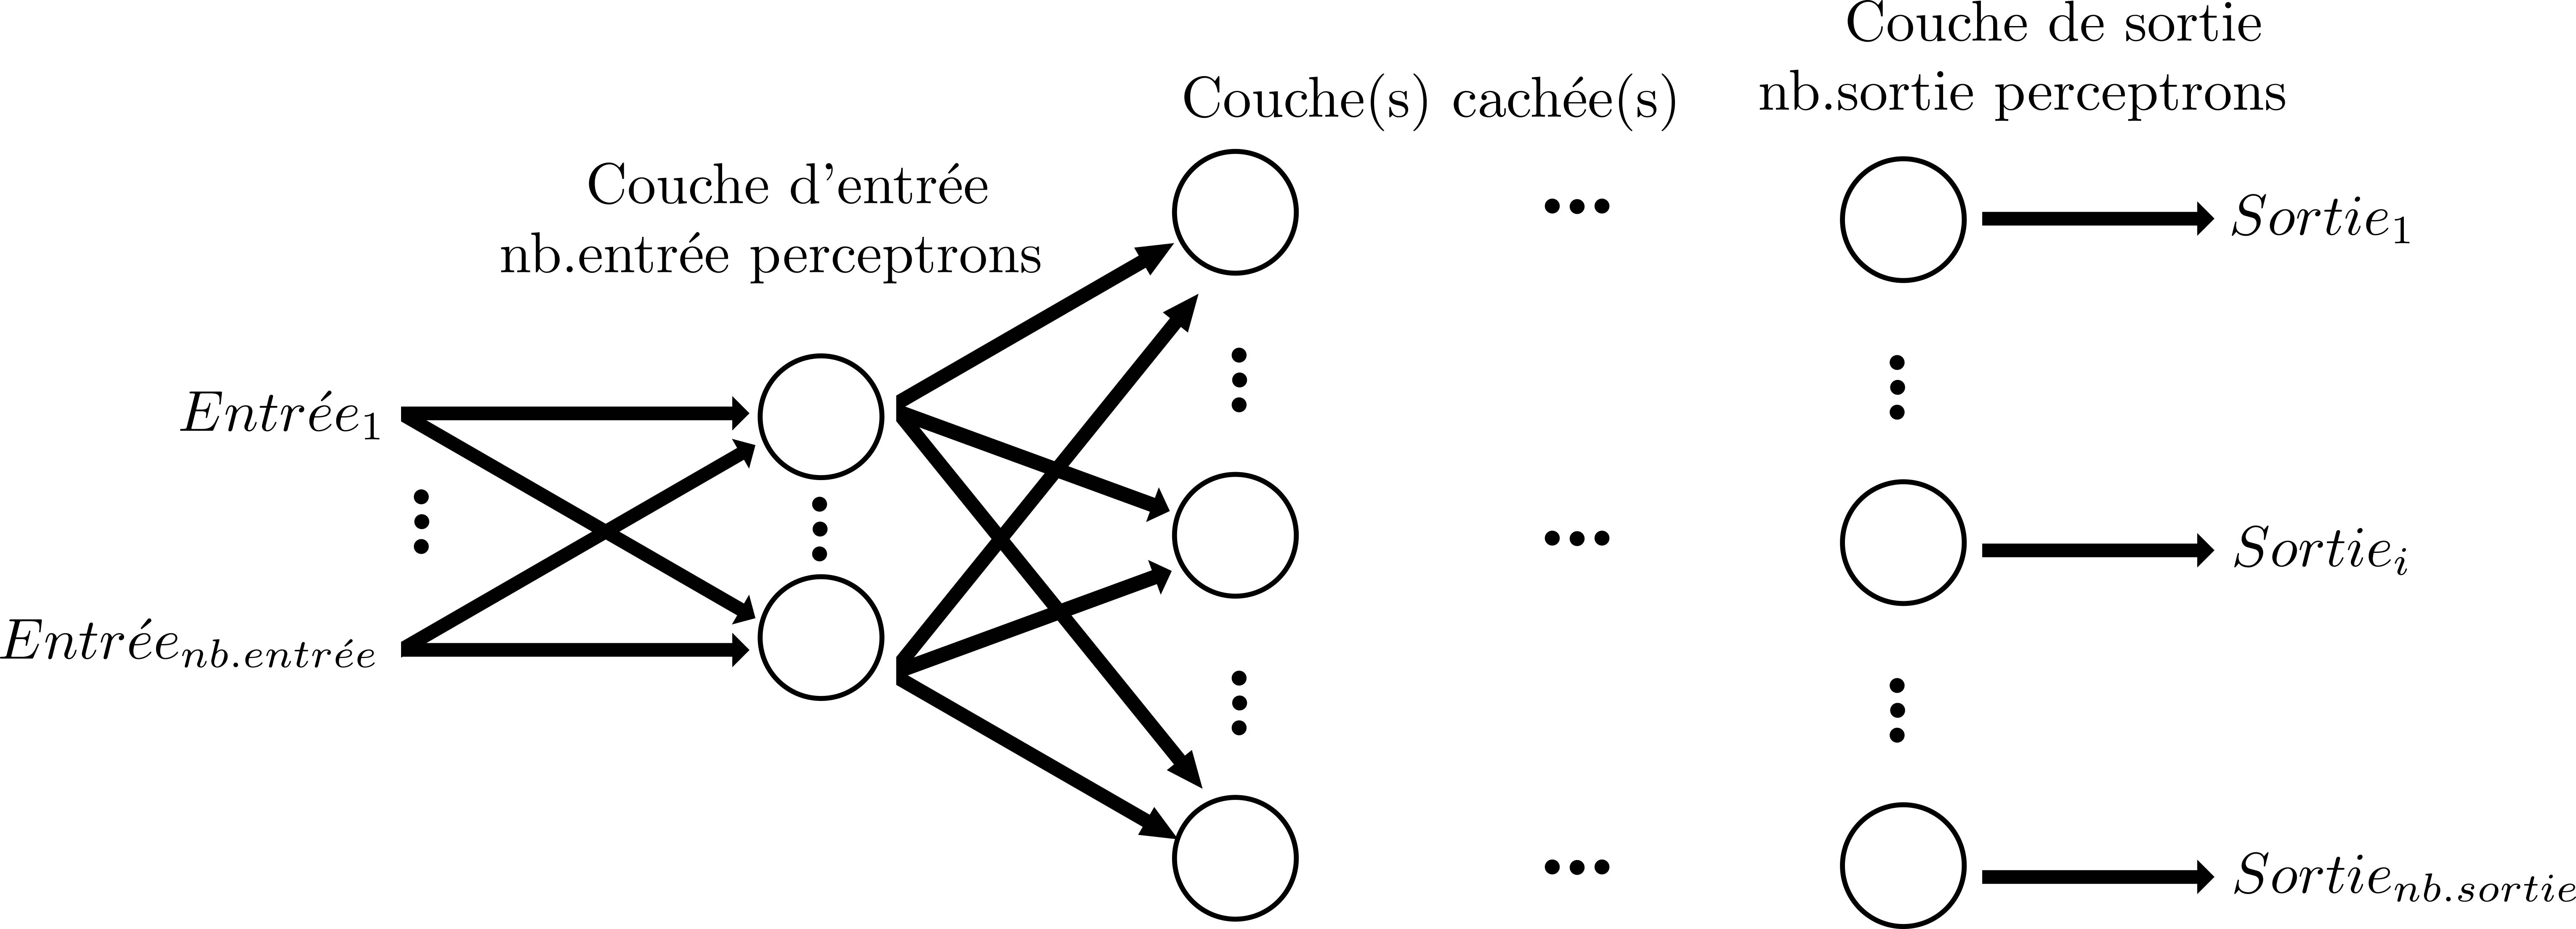
\includegraphics[height=100px]{1-Reseau.png}
	\caption{Schéma d'un réseau de neurones}
\end{figure}
\end{frame}

\begin{frame}{IV - Problème de reproduction de l'opérateur XOR}
\begin{block}{Le XOR nécessite un réseau}
Le XOR, ou exclusif, est un opérateur non linéairement séparable. \\
On peut par exemple démontrer que l'ajout d'une couche cachée de 2 perceptrons suffit à reproduire l'opérateur XOR. \\
\begin{figure}
	\centering
    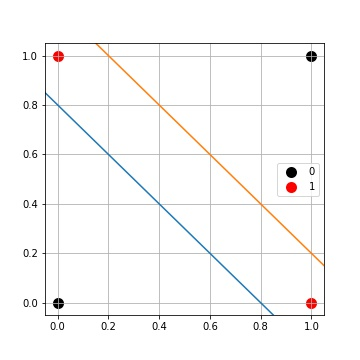
\includegraphics[width=100px]{2-XOR.jpg}
	\caption{Schéma de l'opérateur XOR}
\end{figure}
\end{block}	
\end{frame}

\begin{frame}{IV - Problème de reproduction de l'opérateur XOR}
\begin{figure}
	\centering
    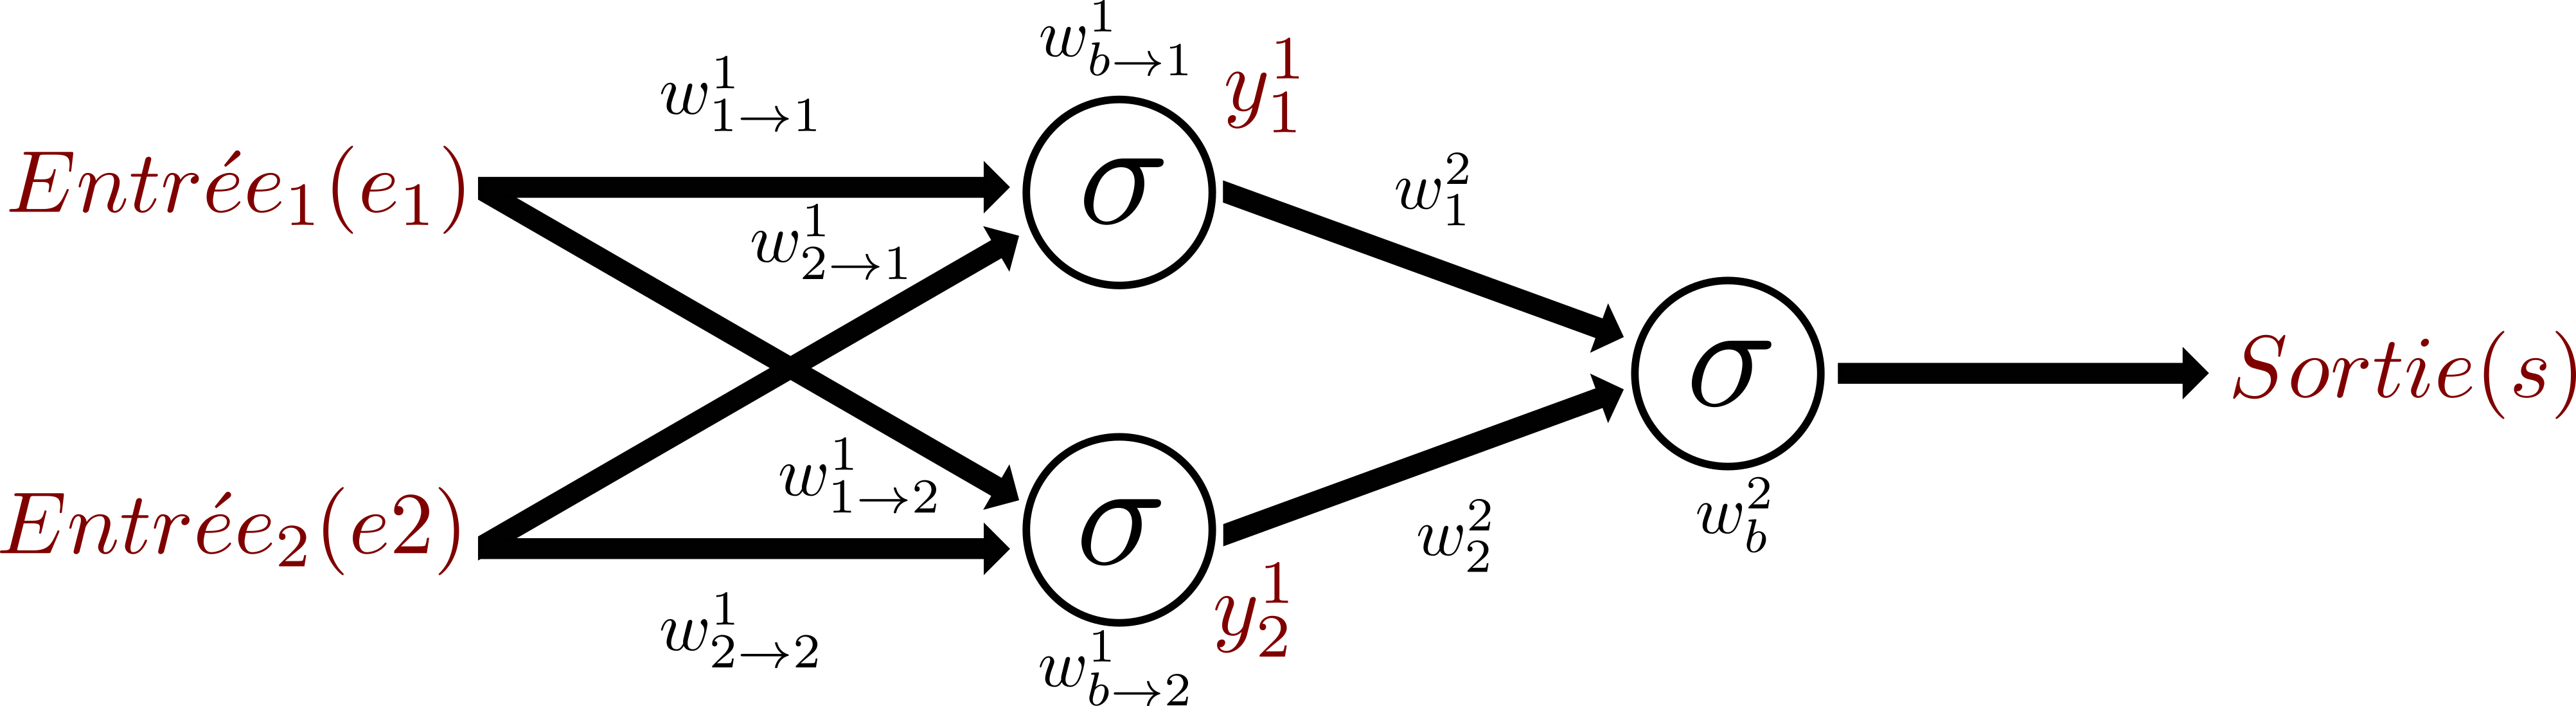
\includegraphics[width=230px]{3-Model.png}
	\caption{Schéma du réseau de neurone reproduisant le XOR}
\end{figure}
\begin{block}{Descente de gradient}
$w \leftarrow w - t \dfrac{\partial f}{\partial w}$ où $t$ est le taux d'apprentissage et $f$ la fonction de coût
\end{block}
\begin{exampleblock}{Exemple}
• $\dfrac{\partial f}{\partial w^2_1} = 2(s - s_{attendue})\sigma_2 'y^1_1$ \\
• $\dfrac{\partial f}{\partial w^1_{1\to 1}} = 2(s - s_{attendue})\sigma_2 'w^2_1 \sigma _{1} ' e_{1}$
\end{exampleblock}

\end{frame}

\begin{frame}
\begin{figure}
	\centering
    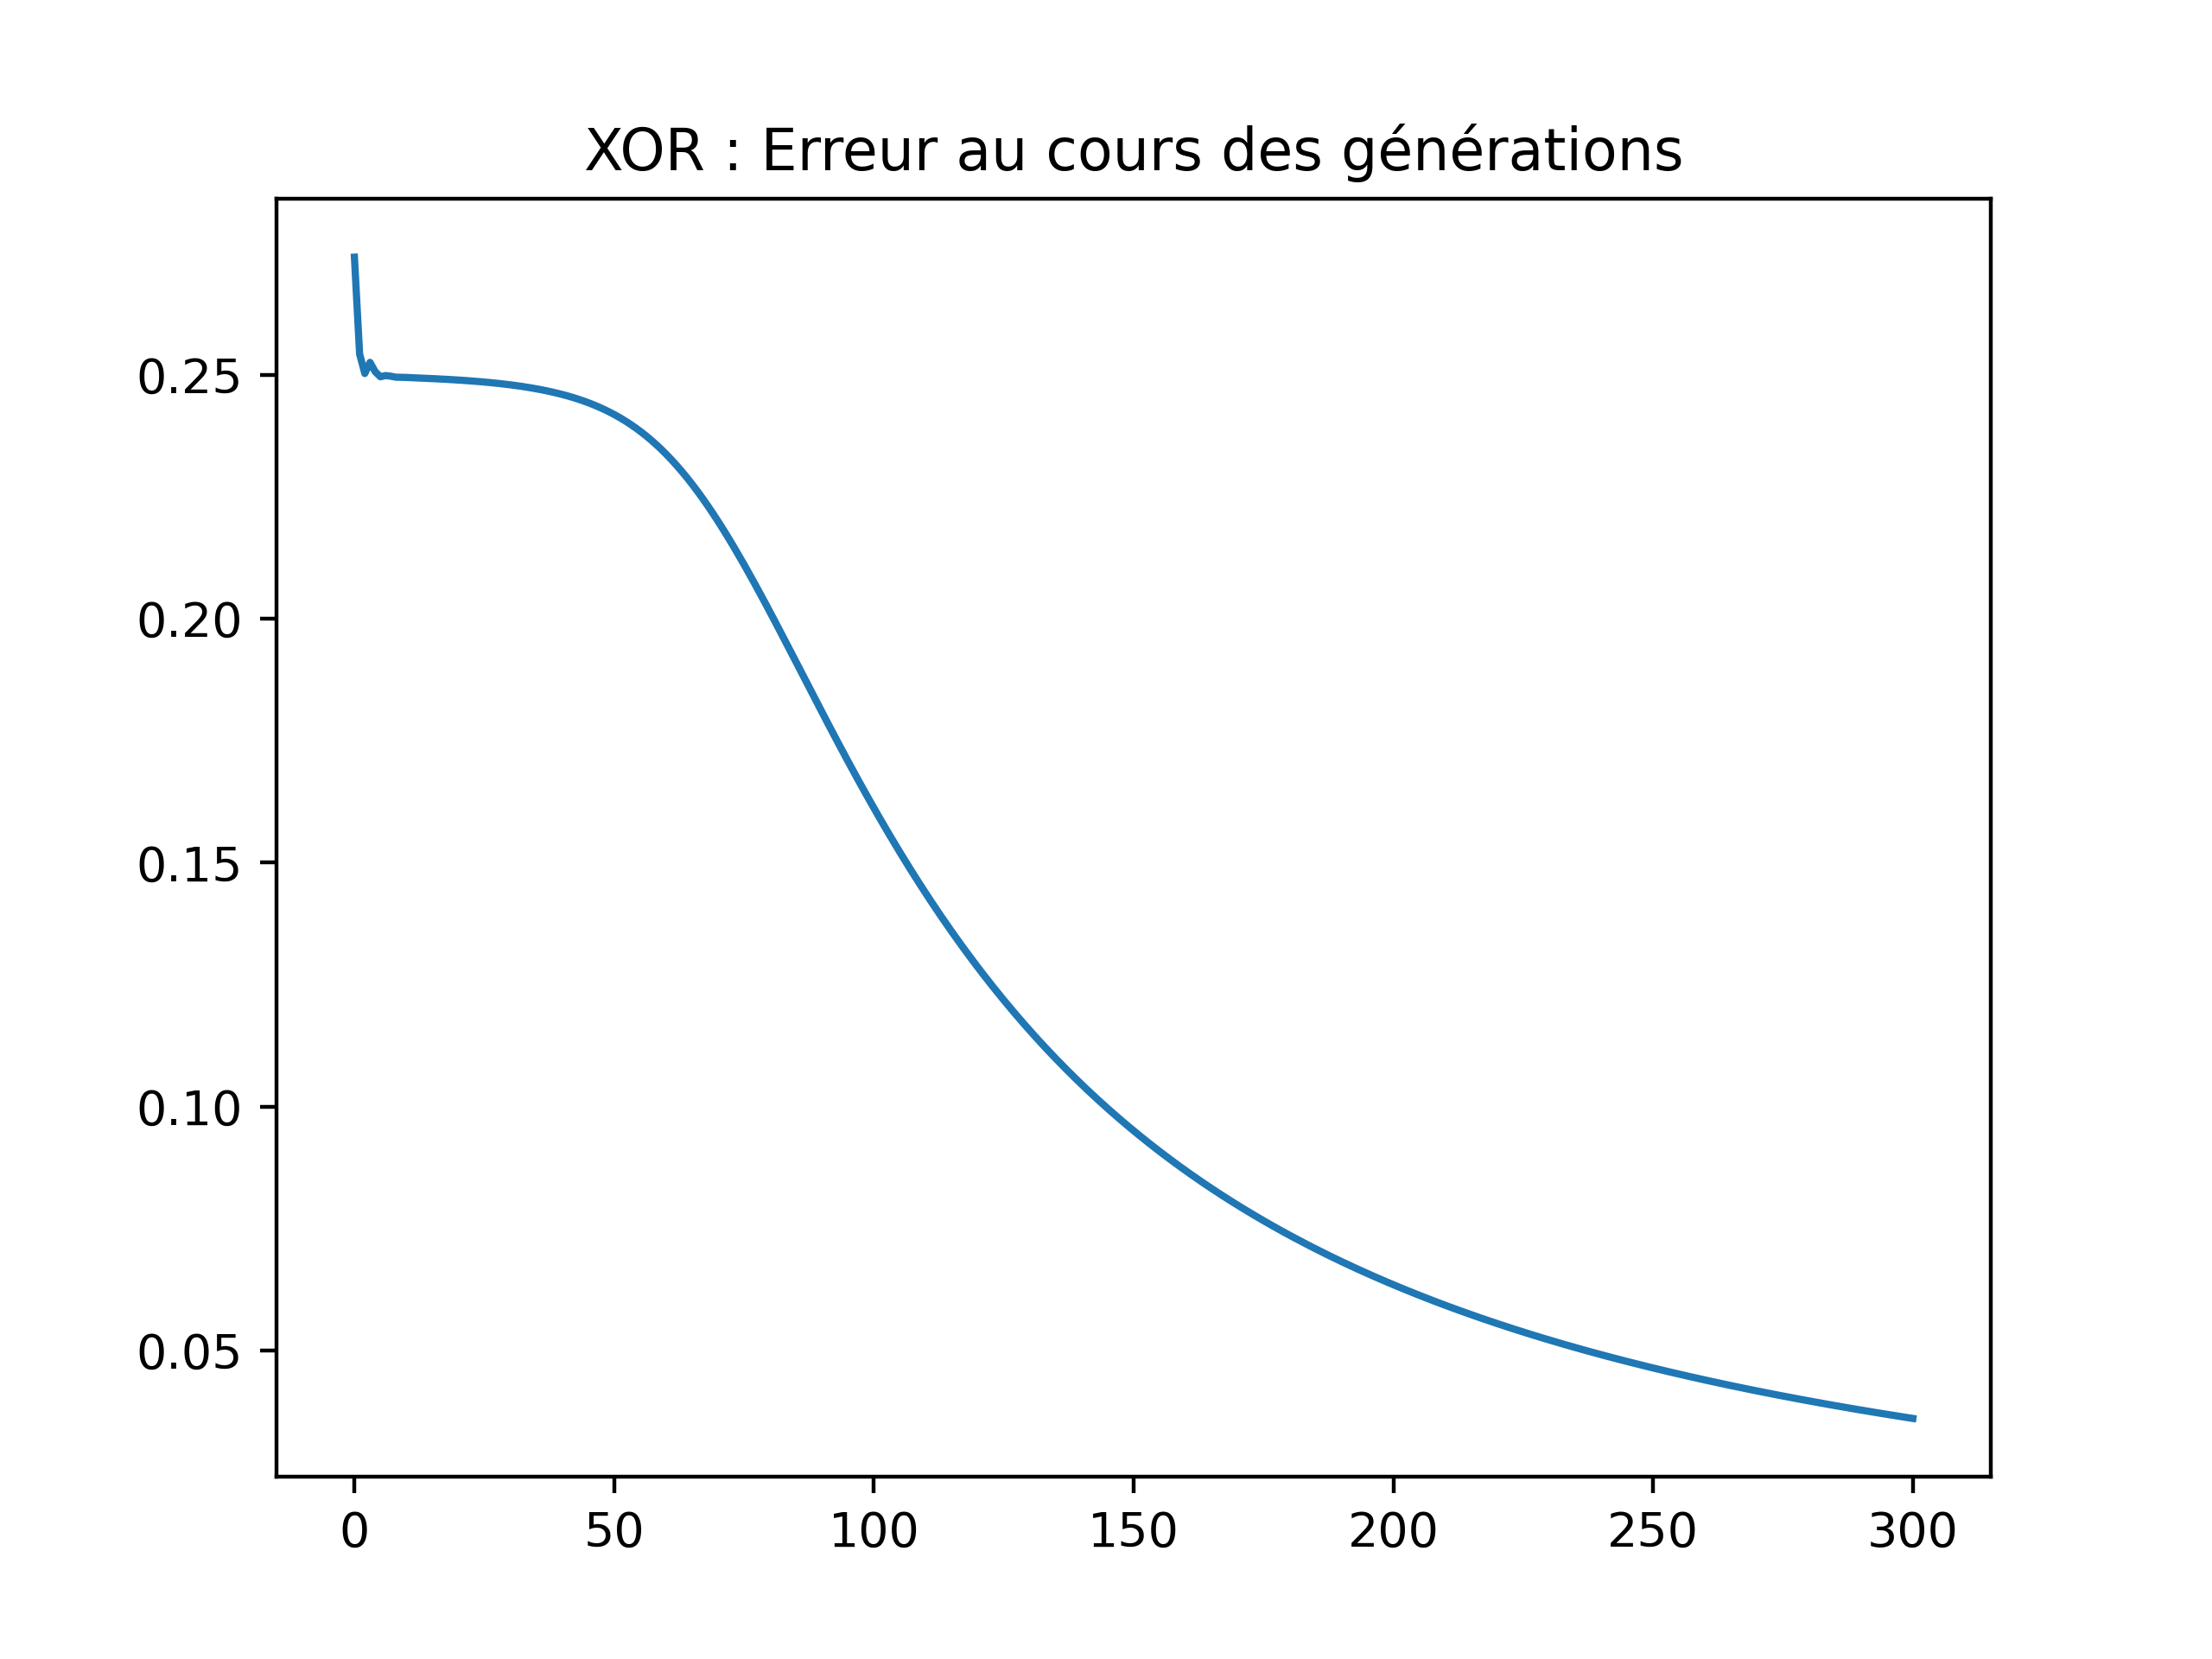
\includegraphics[width=300px]{4-XOR.png}
	\caption{Courbe de décroissance de l'erreur}
\end{figure}
\end{frame}

\begin{frame}{IV - Résultat obtenu}
\begin{block}{Données}
• 4 données \\
• 300 générations \\
• Erreur minimale atteinte 0.036
\end{block}
\begin{align*} 
Entr\acute{e} e\, :
\begin{pmatrix}
0 & 0 \\ 
0 & 1 \\ 
1 & 0 \\ 
1 & 1 
\end{pmatrix} 
		&\to  
\mathlarger{\mathlarger{\sigma_{couche1}}}
\left( \centerdot \times
\begin{pmatrix}
0.85 & 5.42 \\ 
0.85 & 5.40 \\ 
0.14 & 0.44
\end{pmatrix}
\right) \\ 
 		&\to
\mathlarger{\mathlarger{\sigma_{couche2}}}
\left( \centerdot \times
\begin{pmatrix}
-18.39\\ 
14.42 \\ 
0.02
\end{pmatrix}
\right) \\
 		&\to
Sortie\, :
\begin{pmatrix}
0.12 \\ 
0.81 \\ 
0.81 \\ 
0.24
\end{pmatrix}
Sortie_{attendue}\, :
\begin{pmatrix}
0 \\ 
1 \\ 
1 \\ 
0
\end{pmatrix}
\end{align*}
\end{frame}

\section{V - MNIST}
\begin{frame}{V - Reconnaissance d'image}
\begin{block}{Problématique}
On possède une base de données, d'image de chiffres écrit à la main. Ces images sont toutes de taille $28 \times 28$ pixels en noir et blanc. \\
La base de données est divisées en 60000 images pour l'entrainement, et 10000 autres pour la vérification.
\end{block}
\begin{figure}
	\centering
    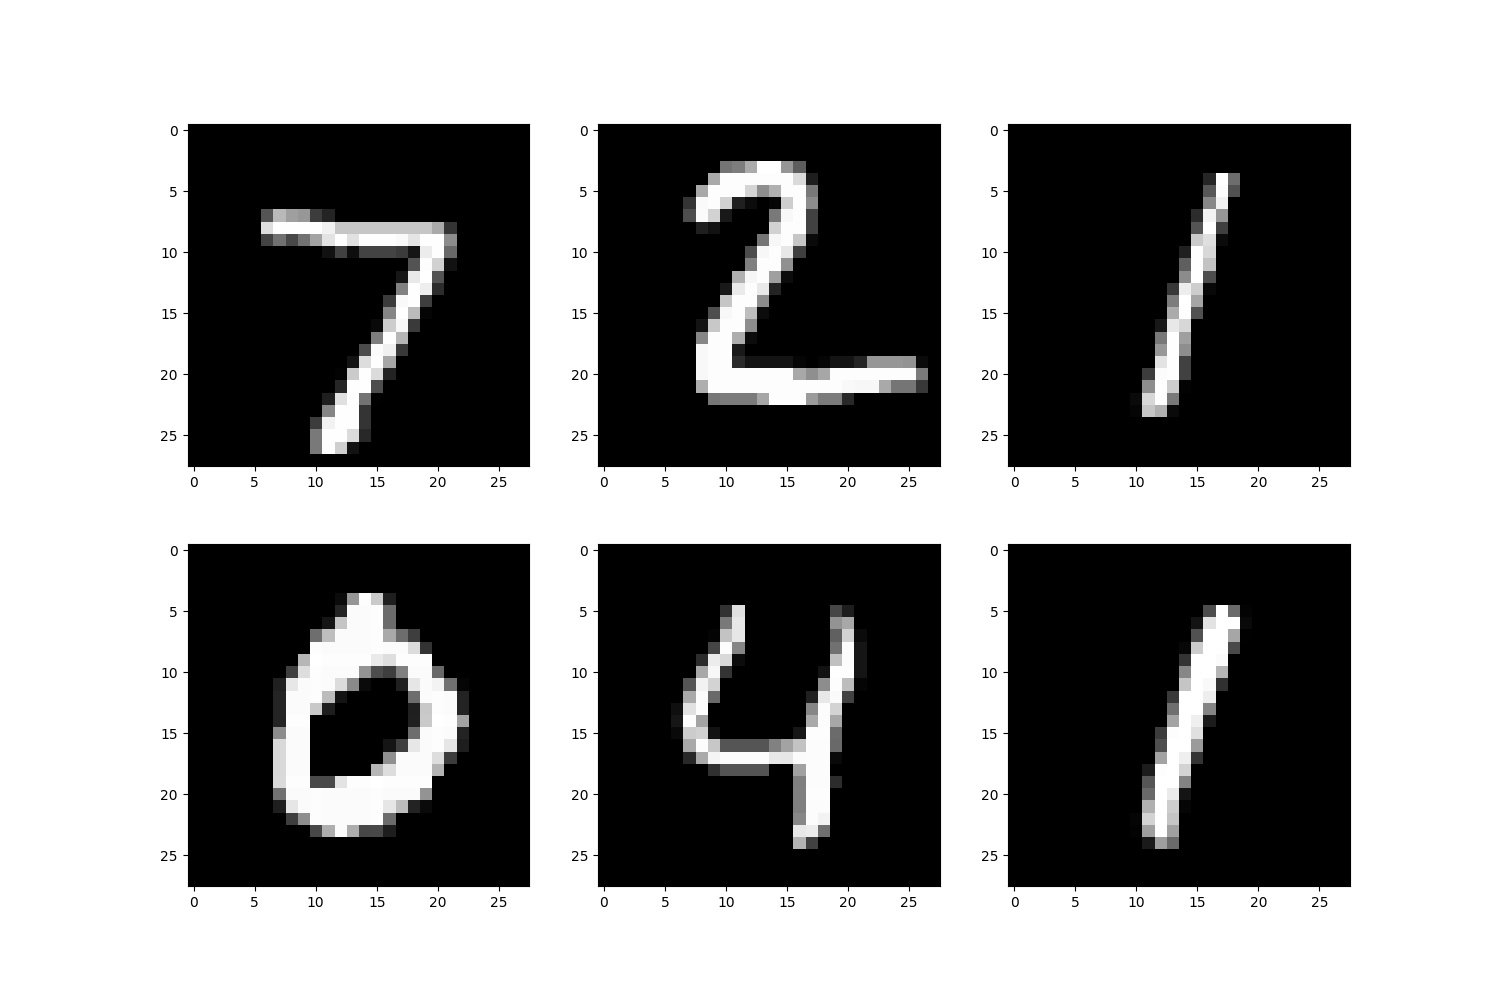
\includegraphics[width=150px]{1-mnist.jpg}
	\caption{Exemple d'images}
\end{figure}
\end{frame}

\begin{frame}{V - Apprentissage d'un problème de classification}
On prend un réseau de neurones avec $28 \times 28 = 784$ entrées, et 10 sorties. \\
\begin{block}{Softmax et Cross-entropy}
Lorsque l'on fait face à un problème de classification, il faut adapter le réseau de neurone. \\
La fonction d'activation softmax est utilisé pour la dernière couche de neurones, elle permet de normaliser les probabilités de sorties. \\
• $p_i = \frac{exp(a_i)}{\sum_{k=1}^{n}exp(e_k)}$ la probabilité de la sortie $a_i$ \\
• $\dfrac{\partial p_i}{\partial a_j} = p_i(\delta_{ij}-p_j)$ \\
La fonction de coût associée est $Cross-entropy$. \\
• $L = -\sum_{k=1}^{n}y_ilog(p_i)$ avec $y_i$ la sortie attendue \\
• $\dfrac{\partial L}{\partial a_i} = p_i - y_i$
\end{block}
\end{frame}

\begin{frame}{V - Softmax}
\begin{figure}
	\centering
    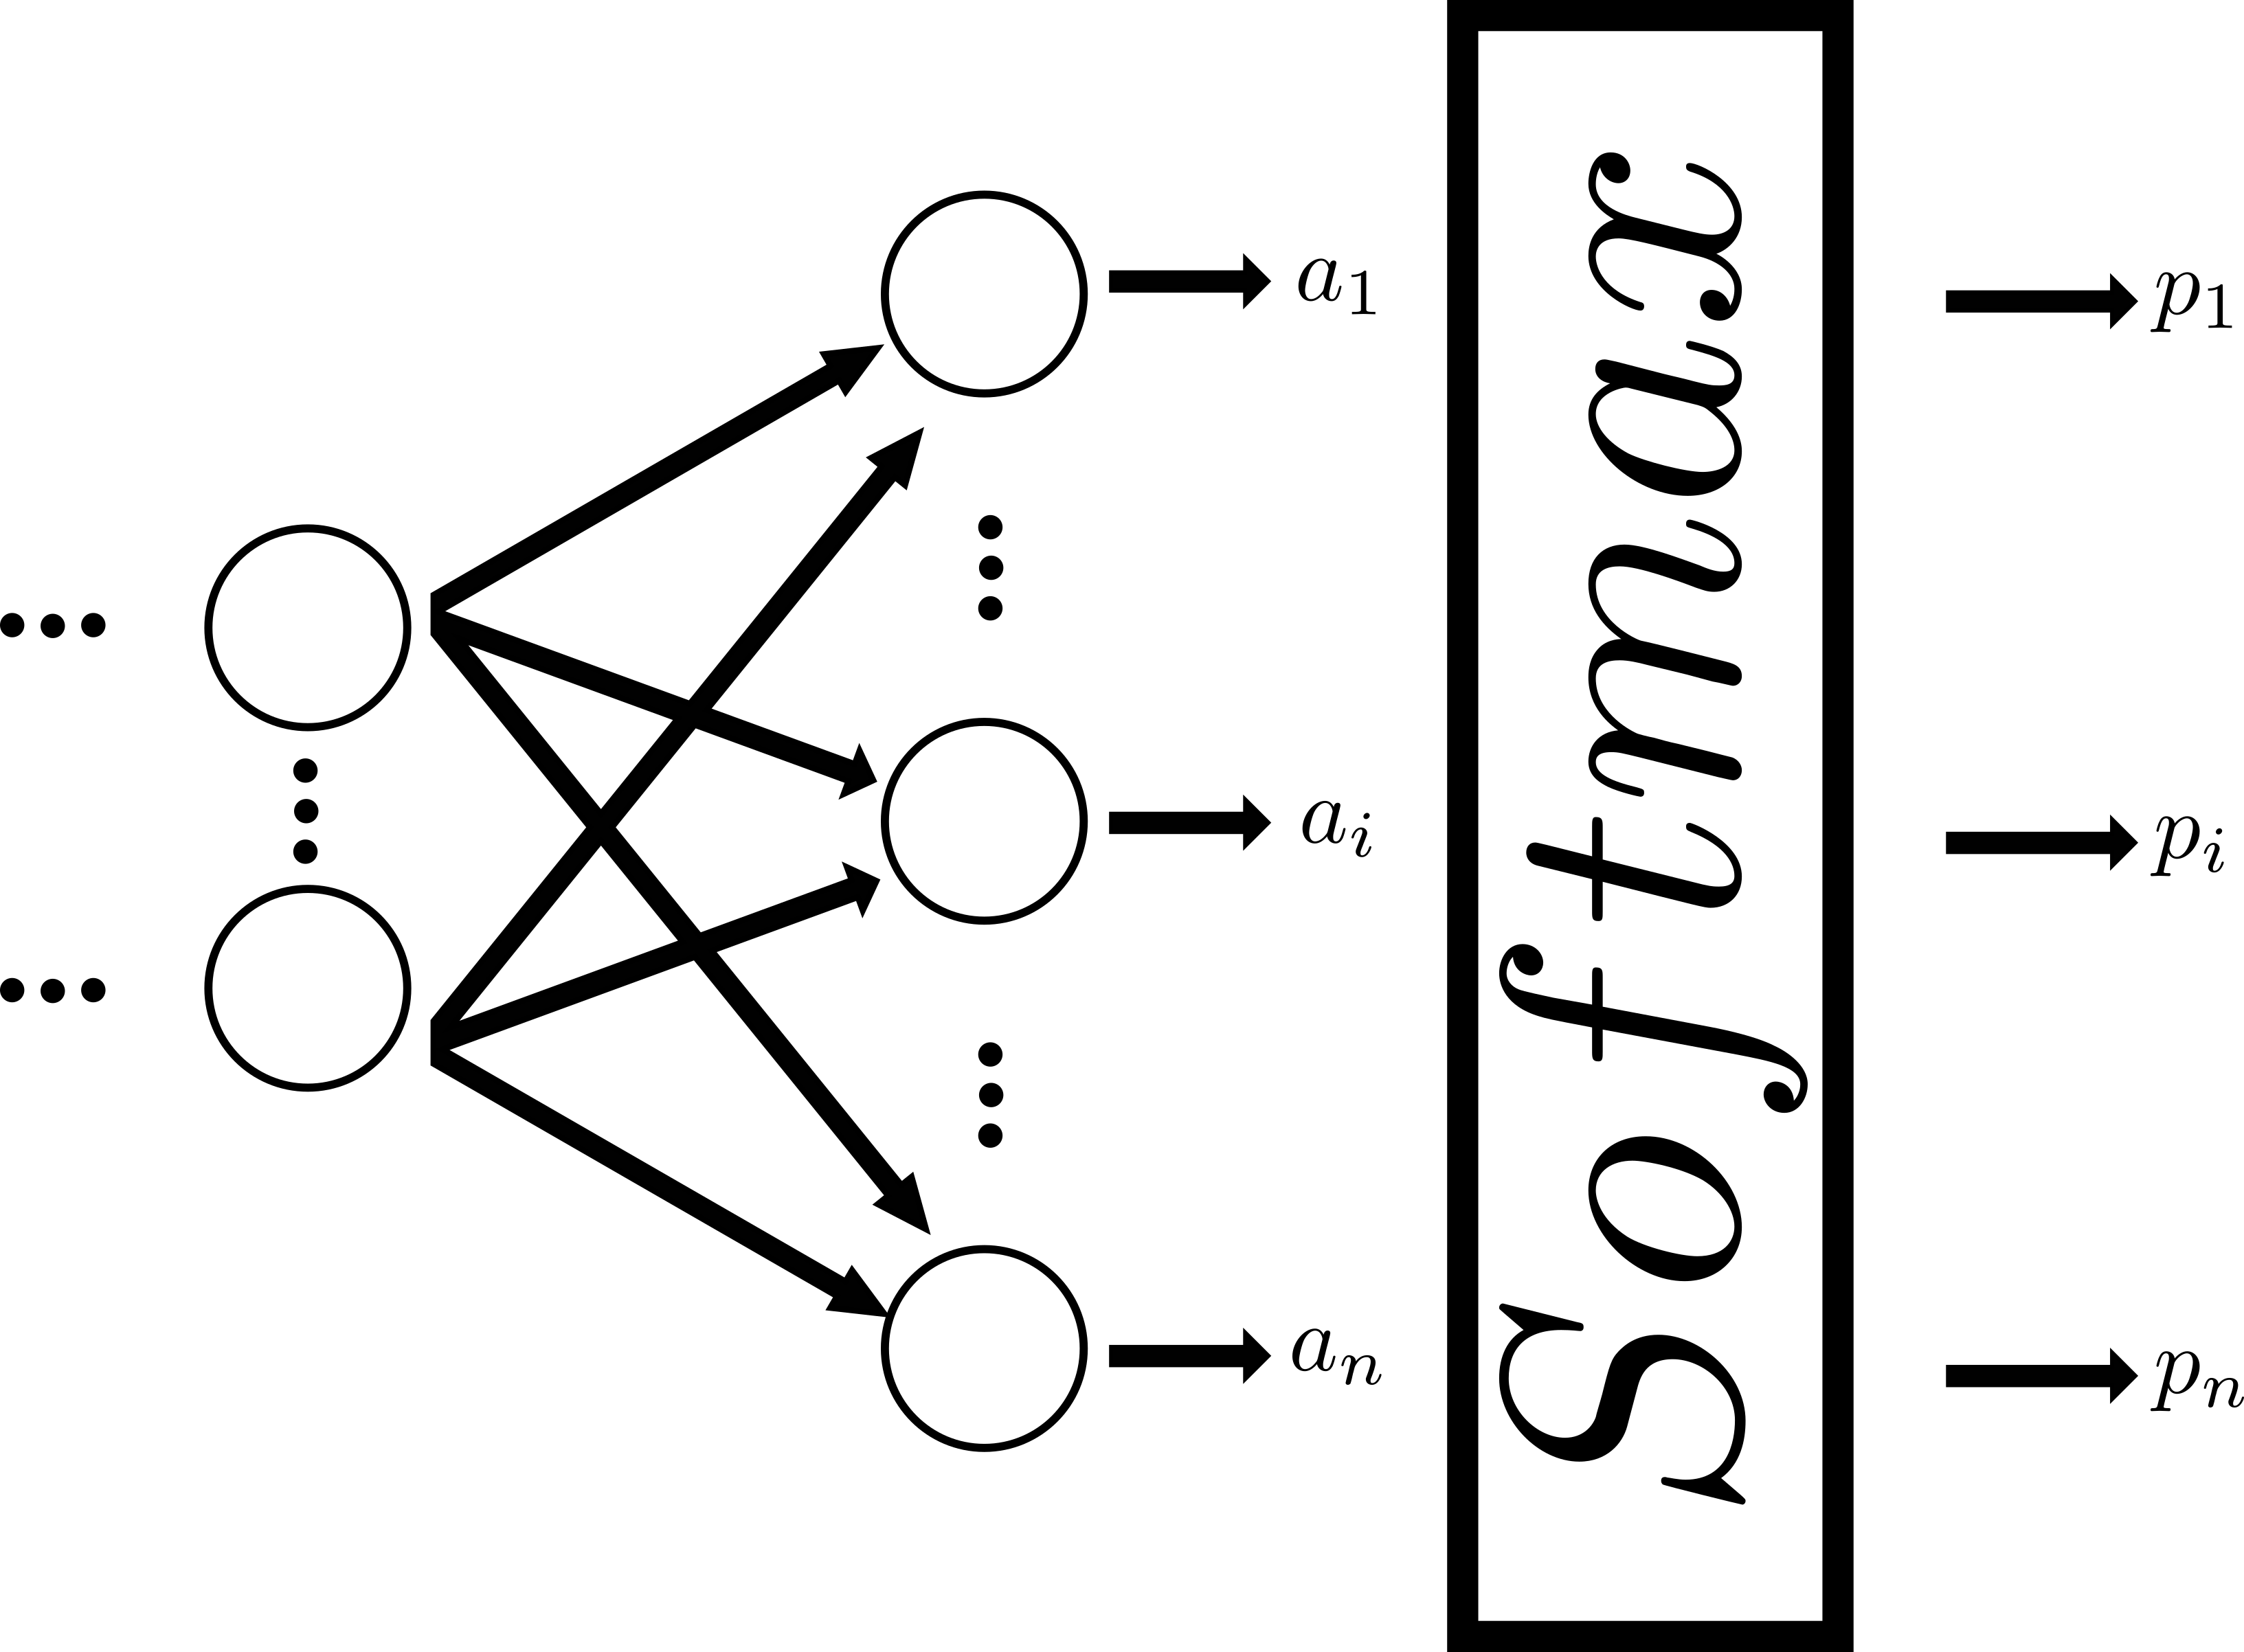
\includegraphics[height=150px]{2-Softmax.png}
	\caption{Schéma d'utilisation du Softmax}
\end{figure}
\end{frame}

\begin{frame}{V - Résultats}
Au terme de 100 générations d'entrainement, on tend à avoir 91.5\% de bonnes réponses sur les données d'entrainement et 91.3\% sur les données de validation. \\
On peut remarquer que dès le début, on à un taux de précision d'environ 10\%, c'est dû au fait que c'est un problème de classification à 10 sorties.
\begin{figure}
	\centering
    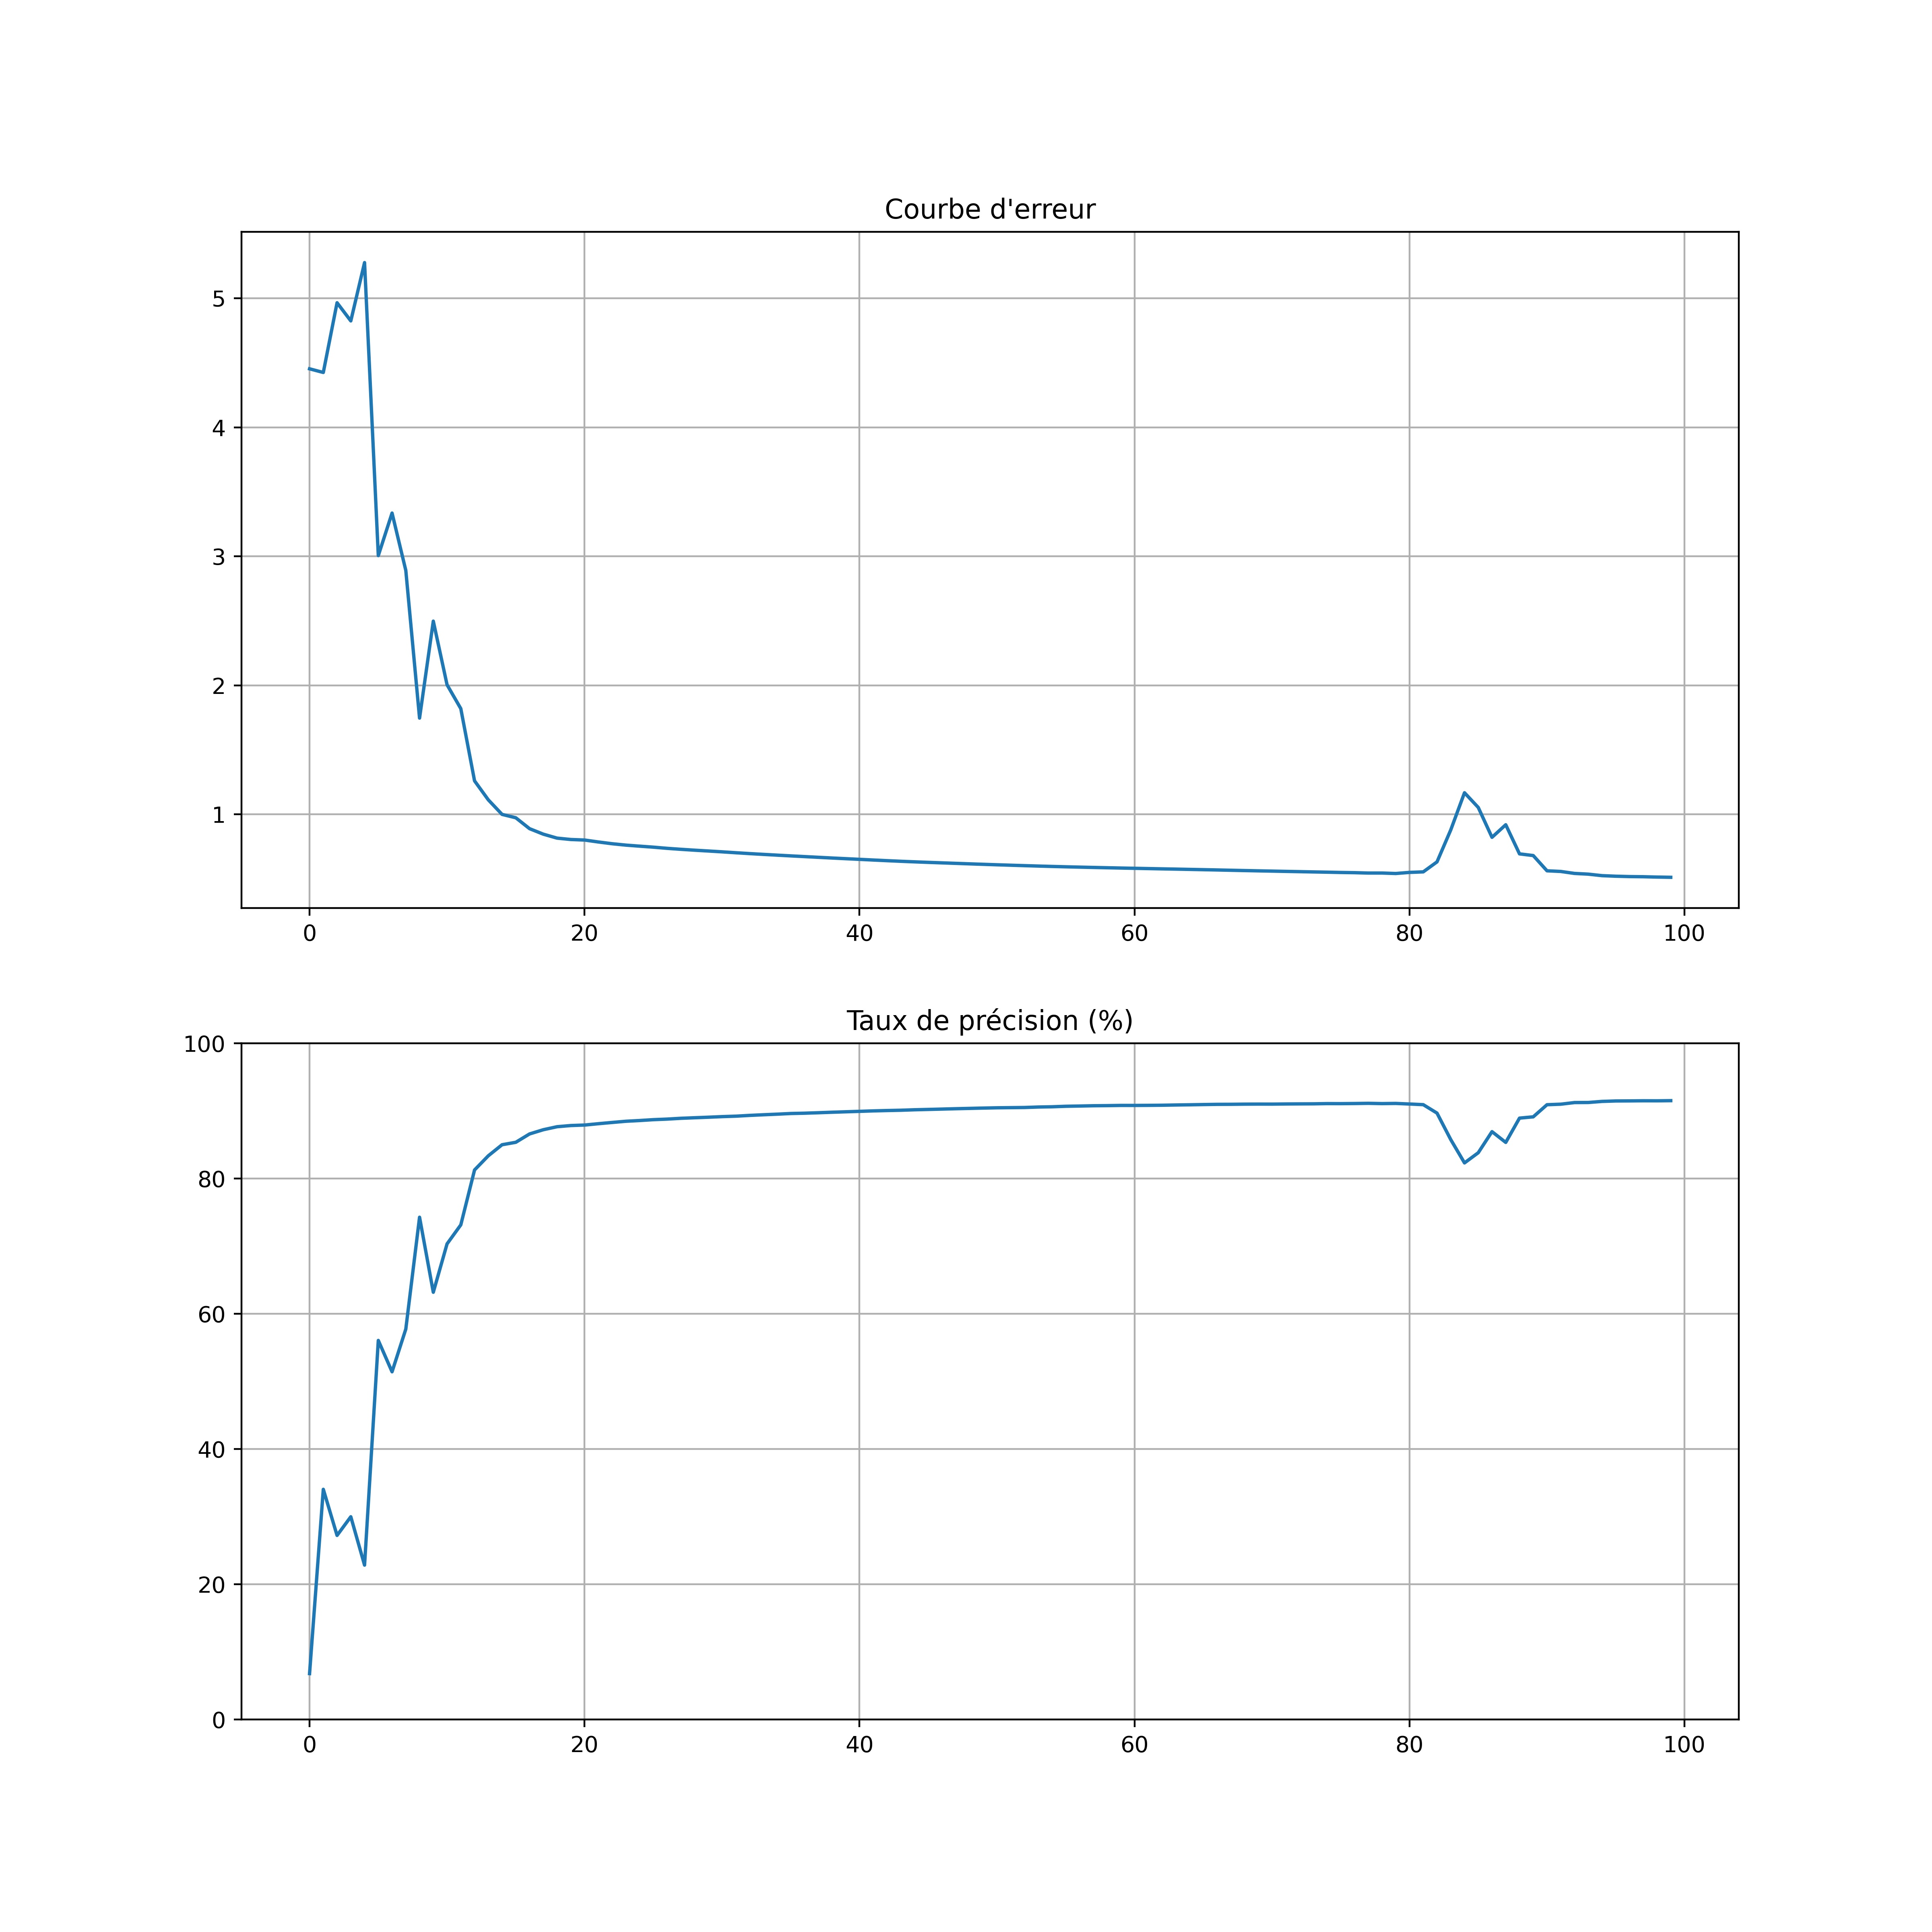
\includegraphics[height=150px]{3-Apprentissage.jpg}
	\caption{Courbes d'apprentissage}
\end{figure}
\end{frame}

\begin{frame}{V - Résultats}
\begin{figure}
	\centering
    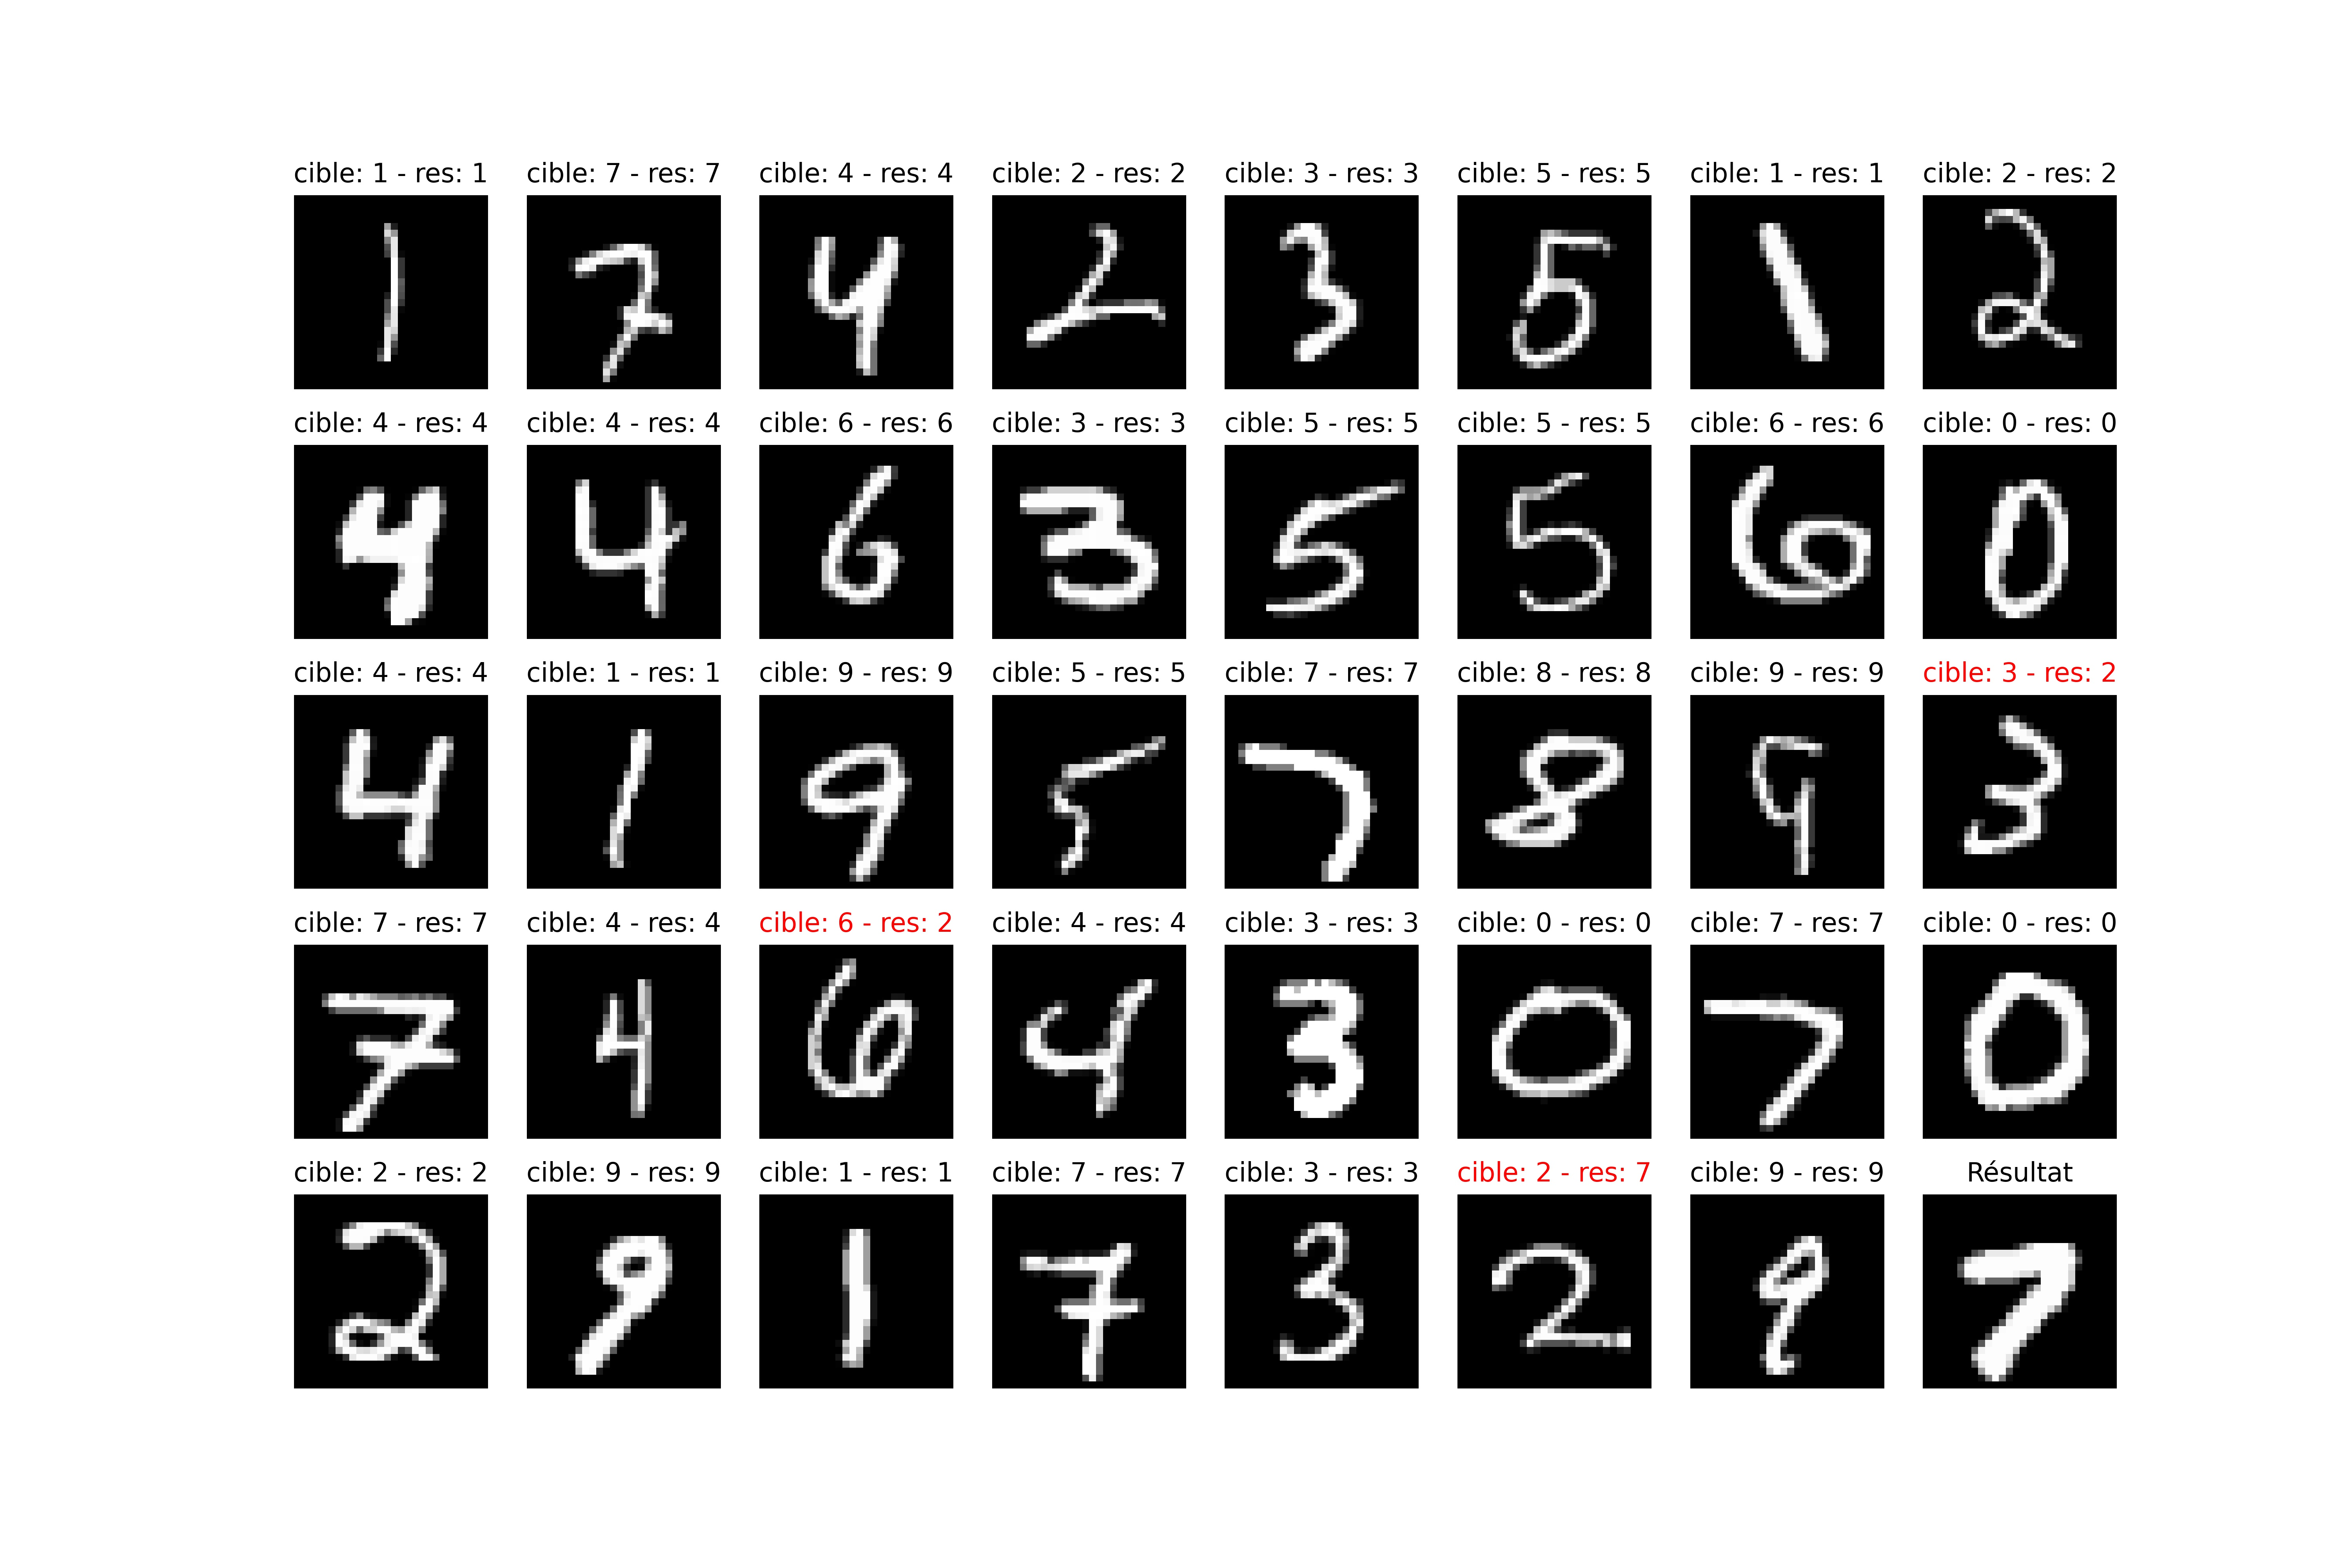
\includegraphics[height=200px]{4-Resultat.jpg}
	\caption{Exemple sur un échantillon de 40 images de validation}
\end{figure}
\end{frame}

\section{VI - Reconnaissance de mot}
\begin{frame}{VI - Reconnaissance de mot}
Un moyen simple de reconnaitre un mot est d'en faire le spectrogramme puis de résoudre le problème de reconnaissance comme si cela était une image. \\
Le site du gouvernement recense ces mots clés pour les appels d'urgences : \\
\begin{enumerate}
  \item[15] malaise, hémorragie, brûlure, intoxication
  \item[17] violences, agression, vol, cambriolage
  \item[18] incendie, gaz, effondrement, électrocution
\end{enumerate}
\begin{figure}
	\begin{subfigure}[]{0.3\textwidth}
		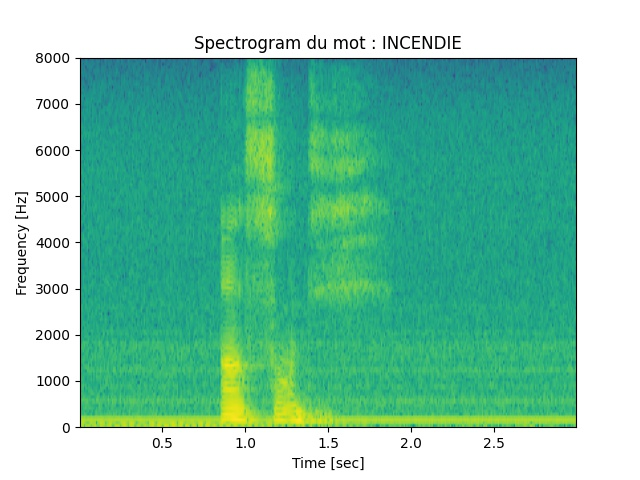
\includegraphics[width=90px]{1-Incendie.jpg}
  		\caption{INCENDIE}
	\end{subfigure}
	\begin{subfigure}[]{0.3\textwidth}
		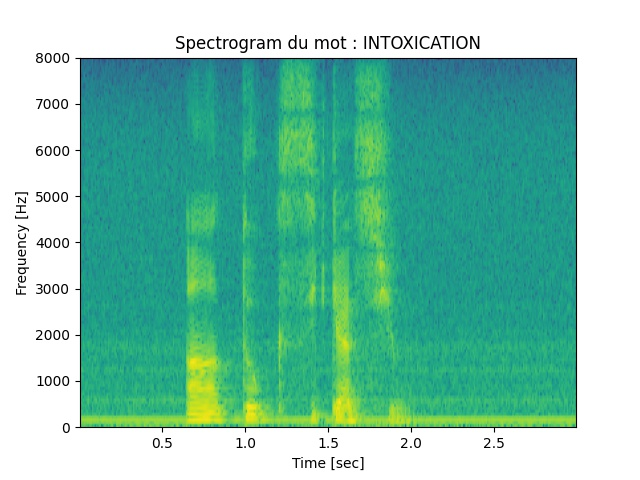
\includegraphics[width=90px]{1-Intoxication.jpg}
  		\caption{INTOXICATION}
	\end{subfigure}
	\begin{subfigure}[]{0.3\textwidth}
		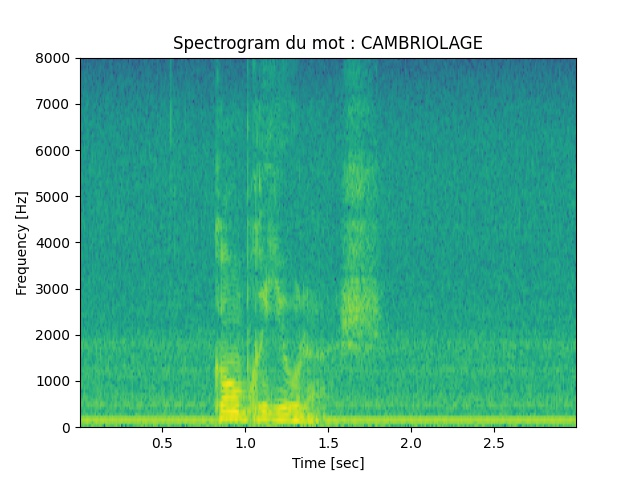
\includegraphics[width=90px]{1-Cambriolage.jpg}
		\caption{CAMBRIOLAGE}
	\end{subfigure}
\end{figure}
\end{frame}

\section{VII - Reconnaissance vocale}
\begin{frame}{VII - Reconnaissance vocale}
Découpage en élément lexicaux, puis décodage du mot.
\begin{figure}
	\begin{subfigure}[]{0.3\textwidth}
		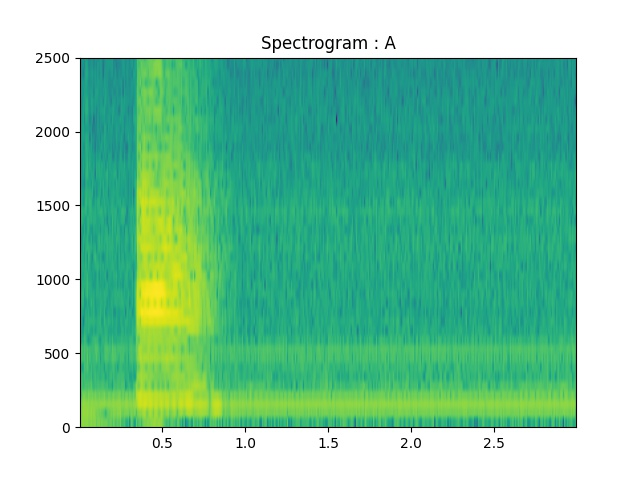
\includegraphics[width=90px]{1-A.jpg}
  		\caption{A}
	\end{subfigure}
	\begin{subfigure}[]{0.3\textwidth}
		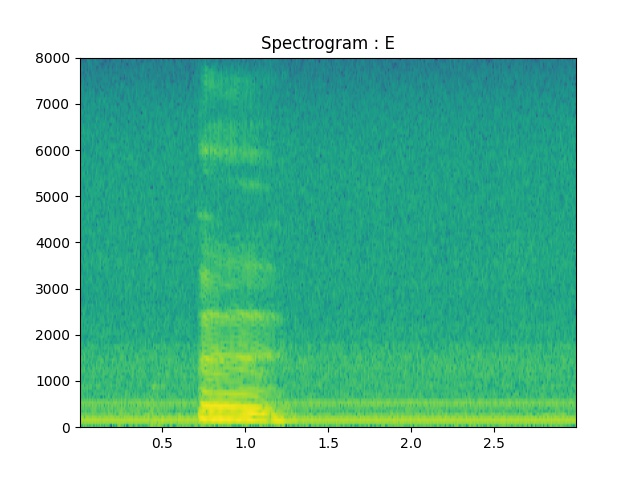
\includegraphics[width=90px]{1-E.jpg}
  		\caption{E}
	\end{subfigure}
	\begin{subfigure}[]{0.3\textwidth}
		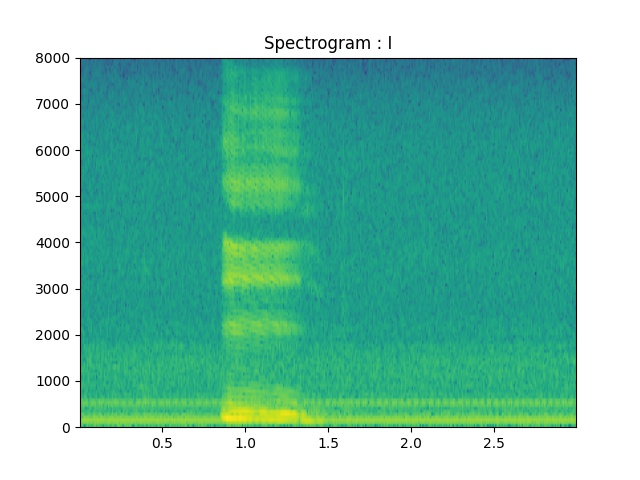
\includegraphics[width=90px]{1-I.jpg}
		\caption{I}
	\end{subfigure}
\end{figure}
\begin{figure}
	\begin{subfigure}[]{0.3\textwidth}
		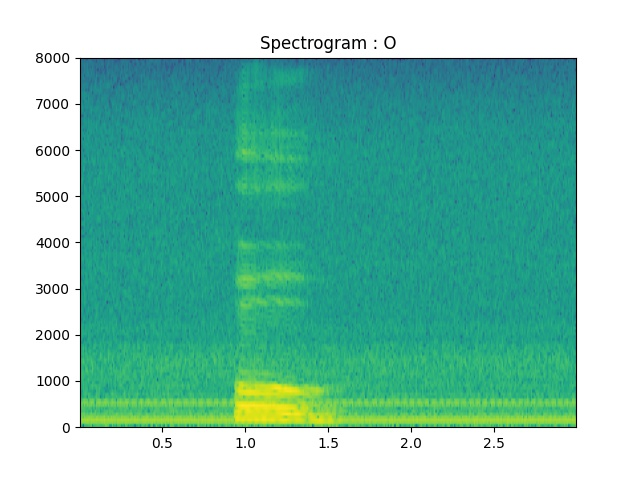
\includegraphics[width=90px]{1-O.jpg}
  		\caption{O}
	\end{subfigure}
	\begin{subfigure}[]{0.3\textwidth}
		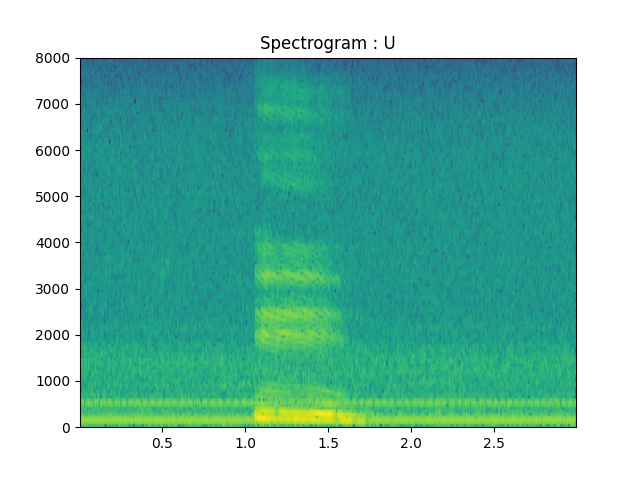
\includegraphics[width=90px]{1-U.jpg}
  		\caption{U}
	\end{subfigure}
	\begin{subfigure}[]{0.3\textwidth}
		
\includegraphics[width=90px]{2-Matching.png}
	\end{subfigure}
\end{figure}
\end{frame}

\end{document}